% Options for packages loaded elsewhere
% Options for packages loaded elsewhere
\PassOptionsToPackage{unicode}{hyperref}
\PassOptionsToPackage{hyphens}{url}
\PassOptionsToPackage{dvipsnames,svgnames,x11names}{xcolor}
%
\documentclass[
  11pt,
  letterpaper,
  DIV=11,
  numbers=noendperiod]{scrartcl}
\usepackage{xcolor}
\usepackage[margin=1in]{geometry}
\usepackage{amsmath,amssymb}
\setcounter{secnumdepth}{5}
\usepackage{iftex}
\ifPDFTeX
  \usepackage[T1]{fontenc}
  \usepackage[utf8]{inputenc}
  \usepackage{textcomp} % provide euro and other symbols
\else % if luatex or xetex
  \usepackage{unicode-math} % this also loads fontspec
  \defaultfontfeatures{Scale=MatchLowercase}
  \defaultfontfeatures[\rmfamily]{Ligatures=TeX,Scale=1}
\fi
\usepackage{lmodern}
\ifPDFTeX\else
  % xetex/luatex font selection
\fi
% Use upquote if available, for straight quotes in verbatim environments
\IfFileExists{upquote.sty}{\usepackage{upquote}}{}
\IfFileExists{microtype.sty}{% use microtype if available
  \usepackage[]{microtype}
  \UseMicrotypeSet[protrusion]{basicmath} % disable protrusion for tt fonts
}{}
\usepackage{setspace}
\makeatletter
\@ifundefined{KOMAClassName}{% if non-KOMA class
  \IfFileExists{parskip.sty}{%
    \usepackage{parskip}
  }{% else
    \setlength{\parindent}{0pt}
    \setlength{\parskip}{6pt plus 2pt minus 1pt}}
}{% if KOMA class
  \KOMAoptions{parskip=half}}
\makeatother
% Make \paragraph and \subparagraph free-standing
\makeatletter
\ifx\paragraph\undefined\else
  \let\oldparagraph\paragraph
  \renewcommand{\paragraph}{
    \@ifstar
      \xxxParagraphStar
      \xxxParagraphNoStar
  }
  \newcommand{\xxxParagraphStar}[1]{\oldparagraph*{#1}\mbox{}}
  \newcommand{\xxxParagraphNoStar}[1]{\oldparagraph{#1}\mbox{}}
\fi
\ifx\subparagraph\undefined\else
  \let\oldsubparagraph\subparagraph
  \renewcommand{\subparagraph}{
    \@ifstar
      \xxxSubParagraphStar
      \xxxSubParagraphNoStar
  }
  \newcommand{\xxxSubParagraphStar}[1]{\oldsubparagraph*{#1}\mbox{}}
  \newcommand{\xxxSubParagraphNoStar}[1]{\oldsubparagraph{#1}\mbox{}}
\fi
\makeatother


\usepackage{longtable,booktabs,array}
\newcounter{none} % for unnumbered tables
\usepackage{calc} % for calculating minipage widths
% Correct order of tables after \paragraph or \subparagraph
\usepackage{etoolbox}
\makeatletter
\patchcmd\longtable{\par}{\if@noskipsec\mbox{}\fi\par}{}{}
\makeatother
% Allow footnotes in longtable head/foot
\IfFileExists{footnotehyper.sty}{\usepackage{footnotehyper}}{\usepackage{footnote}}
\makesavenoteenv{longtable}
\usepackage{graphicx}
\makeatletter
\newsavebox\pandoc@box
\newcommand*\pandocbounded[1]{% scales image to fit in text height/width
  \sbox\pandoc@box{#1}%
  \Gscale@div\@tempa{\textheight}{\dimexpr\ht\pandoc@box+\dp\pandoc@box\relax}%
  \Gscale@div\@tempb{\linewidth}{\wd\pandoc@box}%
  \ifdim\@tempb\p@<\@tempa\p@\let\@tempa\@tempb\fi% select the smaller of both
  \ifdim\@tempa\p@<\p@\scalebox{\@tempa}{\usebox\pandoc@box}%
  \else\usebox{\pandoc@box}%
  \fi%
}
% Set default figure placement to htbp
\def\fps@figure{htbp}
\makeatother





\setlength{\emergencystretch}{3em} % prevent overfull lines

\providecommand{\tightlist}{%
  \setlength{\itemsep}{0pt}\setlength{\parskip}{0pt}}



 


% --- Headings in the teal used by the HTML guide (#07648D) ---
\usepackage{xcolor}
\definecolor{rpteal}{HTML}{07648D}
\addtokomafont{section}{\color{rpteal}}
\addtokomafont{subsection}{\color{rpteal}}
\addtokomafont{subsubsection}{\color{rpteal}}
% --- Map the Unicode symbols this guide uses to LaTeX equivalents. ---
% The remaining glyphs it uses (degree, micro, x, div, en/em dash,
% dagger) are handled natively by the kernel + textcomp.
\usepackage{iftex}
\usepackage{textcomp}
\ifPDFTeX
  % pdflatex: \DeclareUnicodeCharacter lives in inputenc on older
  % LaTeX and in the kernel on newer LaTeX. Load inputenc only if the
  % command is missing, so this works on both without an option clash.
  \ifdefined\DeclareUnicodeCharacter\else\usepackage[utf8]{inputenc}\fi
  \DeclareUnicodeCharacter{2190}{\ensuremath{\leftarrow}}
  \DeclareUnicodeCharacter{2192}{\ensuremath{\rightarrow}}
  \DeclareUnicodeCharacter{2194}{\ensuremath{\leftrightarrow}}
  \DeclareUnicodeCharacter{2264}{\ensuremath{\leq}}
  \DeclareUnicodeCharacter{2265}{\ensuremath{\geq}}
  \DeclareUnicodeCharacter{207A}{\textsuperscript{+}}
  \DeclareUnicodeCharacter{2083}{\textsubscript{3}}
  \DeclareUnicodeCharacter{2084}{\textsubscript{4}}
  \DeclareUnicodeCharacter{26A0}{\textbf{[!]}}
  \DeclareUnicodeCharacter{26A1}{\textbf{[!]}}
\else
  % xelatex / lualatex read UTF-8 natively; remap via newunicodechar.
  \usepackage{newunicodechar}
  \newunicodechar{←}{\ensuremath{\leftarrow}}
  \newunicodechar{→}{\ensuremath{\rightarrow}}
  \newunicodechar{↔}{\ensuremath{\leftrightarrow}}
  \newunicodechar{≤}{\ensuremath{\leq}}
  \newunicodechar{≥}{\ensuremath{\geq}}
  \newunicodechar{⁺}{\textsuperscript{+}}
  \newunicodechar{₃}{\textsubscript{3}}
  \newunicodechar{₄}{\textsubscript{4}}
  \newunicodechar{⚠}{\textbf{[!]}}
  \newunicodechar{⚡}{\textbf{[!]}}
\fi
\KOMAoption{captions}{tableheading}
\makeatletter
\@ifpackageloaded{tcolorbox}{}{\usepackage[skins,breakable]{tcolorbox}}
\@ifpackageloaded{fontawesome5}{}{\usepackage{fontawesome5}}
\definecolor{quarto-callout-color}{HTML}{909090}
\definecolor{quarto-callout-note-color}{HTML}{0758E5}
\definecolor{quarto-callout-important-color}{HTML}{CC1914}
\definecolor{quarto-callout-warning-color}{HTML}{EB9113}
\definecolor{quarto-callout-tip-color}{HTML}{00A047}
\definecolor{quarto-callout-caution-color}{HTML}{FC5300}
\definecolor{quarto-callout-color-frame}{HTML}{acacac}
\definecolor{quarto-callout-note-color-frame}{HTML}{4582ec}
\definecolor{quarto-callout-important-color-frame}{HTML}{d9534f}
\definecolor{quarto-callout-warning-color-frame}{HTML}{f0ad4e}
\definecolor{quarto-callout-tip-color-frame}{HTML}{02b875}
\definecolor{quarto-callout-caution-color-frame}{HTML}{fd7e14}
\makeatother
\makeatletter
\@ifpackageloaded{caption}{}{\usepackage{caption}}
\AtBeginDocument{%
\ifdefined\contentsname
  \renewcommand*\contentsname{Table of contents}
\else
  \newcommand\contentsname{Table of contents}
\fi
\ifdefined\listfigurename
  \renewcommand*\listfigurename{List of Figures}
\else
  \newcommand\listfigurename{List of Figures}
\fi
\ifdefined\listtablename
  \renewcommand*\listtablename{List of Tables}
\else
  \newcommand\listtablename{List of Tables}
\fi
\ifdefined\figurename
  \renewcommand*\figurename{Figure}
\else
  \newcommand\figurename{Figure}
\fi
\ifdefined\tablename
  \renewcommand*\tablename{Table}
\else
  \newcommand\tablename{Table}
\fi
}
\@ifpackageloaded{float}{}{\usepackage{float}}
\floatstyle{ruled}
\@ifundefined{c@chapter}{\newfloat{codelisting}{h}{lop}}{\newfloat{codelisting}{h}{lop}[chapter]}
\floatname{codelisting}{Listing}
\newcommand*\listoflistings{\listof{codelisting}{List of Listings}}
\makeatother
\makeatletter
\makeatother
\makeatletter
\@ifpackageloaded{caption}{}{\usepackage{caption}}
\@ifpackageloaded{subcaption}{}{\usepackage{subcaption}}
\makeatother
\usepackage{bookmark}
\IfFileExists{xurl.sty}{\usepackage{xurl}}{} % add URL line breaks if available
\urlstyle{same}
\hypersetup{
  pdftitle={Puerto Rico Reasonable Potential (RP) Calculator},
  colorlinks=true,
  linkcolor={teal},
  filecolor={Maroon},
  citecolor={Blue},
  urlcolor={teal},
  pdfcreator={LaTeX via pandoc}}


\title{Puerto Rico Reasonable Potential (RP) Calculator}
\usepackage{etoolbox}
\makeatletter
\providecommand{\subtitle}[1]{% add subtitle to \maketitle
  \apptocmd{\@title}{\par {\large #1 \par}}{}{}
}
\makeatother
\subtitle{User Guide}
\author{}
\date{}
\begin{document}
\maketitle

\renewcommand*\contentsname{Contents}
{
\hypersetup{linkcolor=black}
\setcounter{tocdepth}{3}
\tableofcontents
}

\setstretch{1.15}
\section{Overview}\label{sec-overview}

The \textbf{Puerto Rico Reasonable Potential (RP) Calculator} is a
web-based application designed to support EPA Region 2 permit writers in
determining whether reasonable potential (RP) exists for an
NPDES-permitted discharge to cause or contribute to an exceedance of
Puerto Rico's water quality standards (WQS). The application automates
the most data-intensive steps of the RP analysis: retrieving effluent
monitoring data from a local copy of EPA's ICIS-NPDES database, aligning
those data with the applicable Puerto Rico WQS, performing the
statistical projection described in the EPA Technical Support Document
for Water Quality-Based Toxics Control (TSD, 1991) where appropriate,
and generating a documented, reproducible PDF report.

The application is scoped to \textbf{Puerto Rico NPDES permits} and
references the \textbf{Puerto Rico Water Quality Standards Regulation
(PRWQSR), as amended April 2025} (DNER Resolution R-25-006). All numeric
criteria, water classifications, and hardness-dependent metal limits
applied by the app are drawn directly from that regulation.

\begin{tcolorbox}[enhanced jigsaw, arc=.35mm, bottomrule=.15mm, bottomtitle=1mm, breakable, colback=white, colbacktitle=quarto-callout-note-color!10!white, colframe=quarto-callout-note-color-frame, coltitle=black, left=2mm, leftrule=.75mm, opacityback=0, opacitybacktitle=0.6, rightrule=.15mm, title=\textcolor{quarto-callout-note-color}{\faInfo}\hspace{0.5em}{Note}, titlerule=0mm, toprule=.15mm, toptitle=1mm]

\textbf{Where the data come from.} The app does not call a live web
service at analysis time. A companion script (\texttt{refresh\_db.R})
pulls PR/VI facility and DMR records from the ICIS-NPDES Oracle database
on a weekly schedule and writes them to a local SQLite file
(\texttt{data/pr\_rp.sqlite}) that the app reads. This makes the app
fast and reproducible: two analyses run against the same weekly snapshot
return the same result. The refresh date therefore bounds how current
the data can be.

\end{tcolorbox}

\subsection{What the App Does}\label{sec-what-it-does}

For each pollutant and outfall combination at a selected facility, the
app:

\begin{enumerate}
\def\labelenumi{\arabic{enumi}.}
\tightlist
\item
  Retrieves the DMR values whose \textbf{reporting statistic} matches
  what each criterion is written against --- the maximum for most
  ceiling criteria, the minimum for floor criteria such as dissolved
  oxygen and pH, and the geometric mean or 90th percentile for
  interval-based bacteria criteria --- or accepts locally supplied data
\item
  Checks reported units against the WQS unit and converts where a
  conversion is defined
\item
  For criteria evaluated by statistical projection, calculates a
  \textbf{Receiving Water Concentration (RWC)} using the multiplying
  factor (MF) method from TSD Section 3.3.2
\item
  For criteria evaluated by direct comparison, compares the appropriate
  observed statistic to the criterion with no multiplying factor and no
  dilution
\item
  Compares the result to the applicable criterion from the PRWQSR for
  each selected water classification and returns a \textbf{YES / NO /
  DEPENDS} RP determination for each pollutant × outfall × water class
  combination
\item
  Generates a PDF report --- and optionally a ZIP package with
  supporting data --- that documents all inputs, settings, and findings
\end{enumerate}

\begin{tcolorbox}[enhanced jigsaw, arc=.35mm, bottomrule=.15mm, bottomtitle=1mm, breakable, colback=white, colbacktitle=quarto-callout-note-color!10!white, colframe=quarto-callout-note-color-frame, coltitle=black, left=2mm, leftrule=.75mm, opacityback=0, opacitybacktitle=0.6, rightrule=.15mm, title=\textcolor{quarto-callout-note-color}{\faInfo}\hspace{0.5em}{Note}, titlerule=0mm, toprule=.15mm, toptitle=1mm]

\textbf{Not every criterion is a ceiling.} Earlier versions of the app
treated every criterion as a maximum-concentration ceiling to be
projected through the TSD multiplying factor. That is correct for most
pollutants but wrong for several important ones --- dissolved oxygen (a
floor), Enterococci (interval statistics), color and turbidity (direct
comparison), oil \& grease (narrative), and pH and temperature. Each
crosswalk row now declares its own evaluation semantics, so the app
applies the right test to each parameter. Section~\ref{sec-direct}
describes the parameters that are evaluated by direct comparison rather
than projection.

\end{tcolorbox}

\subsection{What the App Does Not Replace}\label{sec-limitations}

The app is an analytical aid, not a substitute for permit writer
judgment. It does not:

\begin{itemize}
\tightlist
\item
  Perform whole effluent toxicity (WET) analysis
\item
  Calculate waste load allocations (WLAs) or mixing zone analyses
\item
  Account for background receiving water concentrations
\item
  Evaluate narrative water quality criteria beyond a simple detection
  screen
\item
  Perform a Streeter-Phelps dissolved-oxygen analysis (see
  Section~\ref{sec-do})
\item
  Replace the fact sheet or other permit development documentation
  requirements
\end{itemize}

When the app returns a YES RP finding, the permit writer must still
determine the appropriate effluent limitation based on the applicable
water quality standard, the dilution ratio, and any mixing zone
authorization. When it returns NO, that finding is based on the
statistical projection or direct comparison alone and should be
considered alongside other factors described in 40 CFR 122.44(d)(1). A
\textbf{DEPENDS} finding means an excursion was not observed but the
absence of one cannot, by itself, rule out reasonable potential for that
parameter (see Section~\ref{sec-interpret-depends} and
Section~\ref{sec-direct}).

\begin{center}\rule{0.5\linewidth}{0.5pt}\end{center}

\section{Regulatory Background}\label{sec-background}

\subsection{Reasonable Potential Under the Clean Water
Act}\label{sec-rp-background}

Under 40 CFR 122.44(d)(1)(i), NPDES permits must include effluent limits
for pollutants that are or may be discharged at levels that will cause,
have the reasonable potential to cause, or contribute to an excursion
above any applicable water quality standard. Determining whether a
discharge has ``reasonable potential'' is therefore a required step in
permit development for any parameter that is monitored at an outfall.

EPA's 1991 Technical Support Document for Water Quality-Based Toxics
Control (TSD) provides the recommended methodology for making this
determination using effluent monitoring data. The core question is
whether the upper bound of the expected effluent concentration
distribution, projected into the receiving water accounting for
dilution, could exceed the applicable criterion. The statistical
approach in the TSD uses the coefficient of variation (CV) of the
effluent data and the number of samples to construct this projection,
with the lognormal distribution used as the basis for the multiplying
factors.

\subsection{The Puerto Rico Water Quality Standards
Regulation}\label{sec-prwqs}

The PRWQSR, administered by Puerto Rico's Department of Natural and
Environmental Resources (DNER), establishes the water quality standards
that NPDES permits in Puerto Rico must protect. The regulation
classifies Puerto Rico's waters by designated use and sets numeric
criteria for a wide range of pollutants. The 2025 amendment (Resolution
R-25-006, effective June 27, 2025) is the currently applicable version.

The standards that drive RP determinations fall into several categories
as implemented in the app:

\begin{itemize}
\tightlist
\item
  \textbf{Fixed numeric criteria} --- a single concentration limit for a
  given pollutant and water classification (e.g., arsenic in Class SB at
  36 µg/L)
\item
  \textbf{Hardness-dependent criteria} --- applicable to seven metals in
  Class SD waters; the criterion is computed from the receiving water
  hardness using regression equations specified in Rule 1303.1(J)(1)
  (see Section~\ref{sec-metals})
\item
  \textbf{Condition-dependent criteria} --- applicable to Total Ammonia
  Nitrogen (TAN) in Class SD waters; the criterion varies with receiving
  water pH and temperature as specified in Rule 1303.2(C)(2)(l) (see
  Section~\ref{sec-tan})
\item
  \textbf{Range and floor criteria} --- pH must stay within a range, and
  dissolved oxygen must stay above a floor. These are evaluated by
  direct comparison, not projection (see Section~\ref{sec-direct})
\item
  \textbf{Interval and narrative criteria} --- Enterococci criteria are
  frequency- and interval-based statistics, and oil \& grease is a
  narrative ``substantially free from'' standard (see
  Section~\ref{sec-entero} and Section~\ref{sec-oil})
\end{itemize}

Three Class SD parameters --- total nitrogen, total phosphorus, and
selenium --- carry \textbf{separate criteria depending on whether the
receiving water is a stream or a reservoir/lake}. The app reports these
as distinct water-class lines (e.g., \emph{class SD waters --- stream}
vs \emph{class SD waters --- reservoir/lake}) so the permit writer can
see which receiving-water type drives a finding.

\subsection{Water Classifications Relevant to NPDES
Permitting}\label{sec-classifications}

The PRWQSR classifies Puerto Rico's waters into several categories. The
app includes the four classifications most relevant to NPDES point
source discharges. Understanding these classifications is important
because the applicable criterion --- and therefore the RP determination
--- differs by classification.

\textbf{Class SB --- Coastal and Estuarine Waters} Class SB encompasses
all coastal and estuarine waters of Puerto Rico not designated as the
more protective Class SA (which includes the bioluminescent lagoons and
other waters of exceptional ecological value where point source
discharges are not permitted). Class SB extends from mean sea level to a
maximum of approximately 10.35 miles offshore and includes associated
wetlands. Designated uses include primary and secondary contact
recreation, and propagation and maintenance of desirable species
including threatened and endangered species. Most NPDES-permitted
facilities discharging to coastal waters in Puerto Rico discharge to
Class SB receiving waters.

\textbf{Class SD --- Surface Waters} Class SD covers all surface waters
of Puerto Rico --- streams, rivers, lakes, reservoirs, and inland water
bodies --- except those designated as the more protective Class SE
(Laguna Tortuguero and Laguna Cartagena). Designated uses include use as
a raw source of public water supply, propagation and maintenance of
desirable species, and primary and secondary contact recreation. Class
SD criteria are generally more stringent than Class SB for most
parameters because of the drinking water supply designation. Several
criteria under Class SD depend on receiving water hardness (for metals)
or on pH and temperature (for TAN), and a few distinguish stream from
reservoir/lake receiving waters.

\textbf{Class SG --- Ground Waters} Class SG includes all ground waters
of Puerto Rico, including those that discharge into coastal, surface,
and estuarine waters. Designated uses are drinking water supply and
agricultural use including irrigation. Ground water criteria are
typically the drinking water (DW) or human health (HH) values, whichever
is more stringent given the receiving water body into which the ground
water flows.

\textbf{Surface Waters (general)} In the app's water type filter,
``Surface Waters'' maps to the PRWQSR's general surface water standards
(Rule 1303.1) that apply across all surface water classifications, as
distinct from the class-specific criteria under Rule 1303.2. The general
standards include temperature, asbestos, radium-226, strontium-90, gross
beta, and oil \& grease.

\begin{tcolorbox}[enhanced jigsaw, arc=.35mm, bottomrule=.15mm, bottomtitle=1mm, breakable, colback=white, colbacktitle=quarto-callout-note-color!10!white, colframe=quarto-callout-note-color-frame, coltitle=black, left=2mm, leftrule=.75mm, opacityback=0, opacitybacktitle=0.6, rightrule=.15mm, title=\textcolor{quarto-callout-note-color}{\faInfo}\hspace{0.5em}{Note}, titlerule=0mm, toprule=.15mm, toptitle=1mm]

\textbf{Selecting water classifications in the app:} The water
classification selection determines which WQS rows from the crosswalk
are active for both data filtering and RP comparison. Selecting multiple
classifications produces RP determinations for each class independently
--- the app reports a ``worst-case'' RP across all selected classes, as
well as the per-class breakdown. The general-standard parameters
(temperature, oil \& grease, and the others listed above) appear
\textbf{only} when ``Surface Waters'' or ``All'' is selected ---
narrowing to a single specific class will not pull them in. When in
doubt about which classification applies to a receiving water body,
consult the PRWQSR classification maps (Rule 1302) or contact the DNER
Water Quality Program.

\end{tcolorbox}

\begin{center}\rule{0.5\linewidth}{0.5pt}\end{center}

\section{Getting Started}\label{sec-getting-started}

\subsection{Two Workflows at a Glance}\label{sec-workflows}

The app offers two entry points depending on whether the facility
appears in the local ICIS-NPDES database.

{\def\LTcaptype{none} % do not increment counter
\begin{longtable}[]{@{}
  >{\raggedright\arraybackslash}p{(\linewidth - 4\tabcolsep) * \real{0.3333}}
  >{\raggedright\arraybackslash}p{(\linewidth - 4\tabcolsep) * \real{0.3333}}
  >{\raggedright\arraybackslash}p{(\linewidth - 4\tabcolsep) * \real{0.3333}}@{}}
\toprule\noalign{}
\begin{minipage}[b]{\linewidth}\raggedright
\end{minipage} & \begin{minipage}[b]{\linewidth}\raggedright
\textbf{NPDES Workflow}
\end{minipage} & \begin{minipage}[b]{\linewidth}\raggedright
\textbf{Standalone Workflow}
\end{minipage} \\
\midrule\noalign{}
\endhead
\bottomrule\noalign{}
\endlastfoot
\textbf{Best for} & Existing permitted facilities & New permits,
reissuances with no prior ID, or supplementing the database with local
measurements \\
\textbf{Data source} & Local ICIS-NPDES database (weekly refresh) &
User-supplied CSV using the app's template \\
\textbf{Requires} & NPDES permit ID & Completed DMR template \\
\textbf{Can supplement with local data} & Yes --- via the Append DMR
function & N/A --- local data is the primary source \\
\end{longtable}
}

Both workflows share the same Analysis Settings, Findings, and Report
pages. The only difference is how effluent data are loaded.

\subsection{Navigating the App}\label{sec-navigation}

The app uses a single-page layout with page routing. A persistent top
bar appears on every page with a \textbf{← Back to Start} button
(returns to the landing page) and a \textbf{User Guide} button (opens
this document in a modal window). Within each page you also move using
contextual buttons (e.g., ``← Back to Search,'' ``← Back to Settings,''
``Return Home'').

\begin{figure}[H]

{\centering \pandocbounded{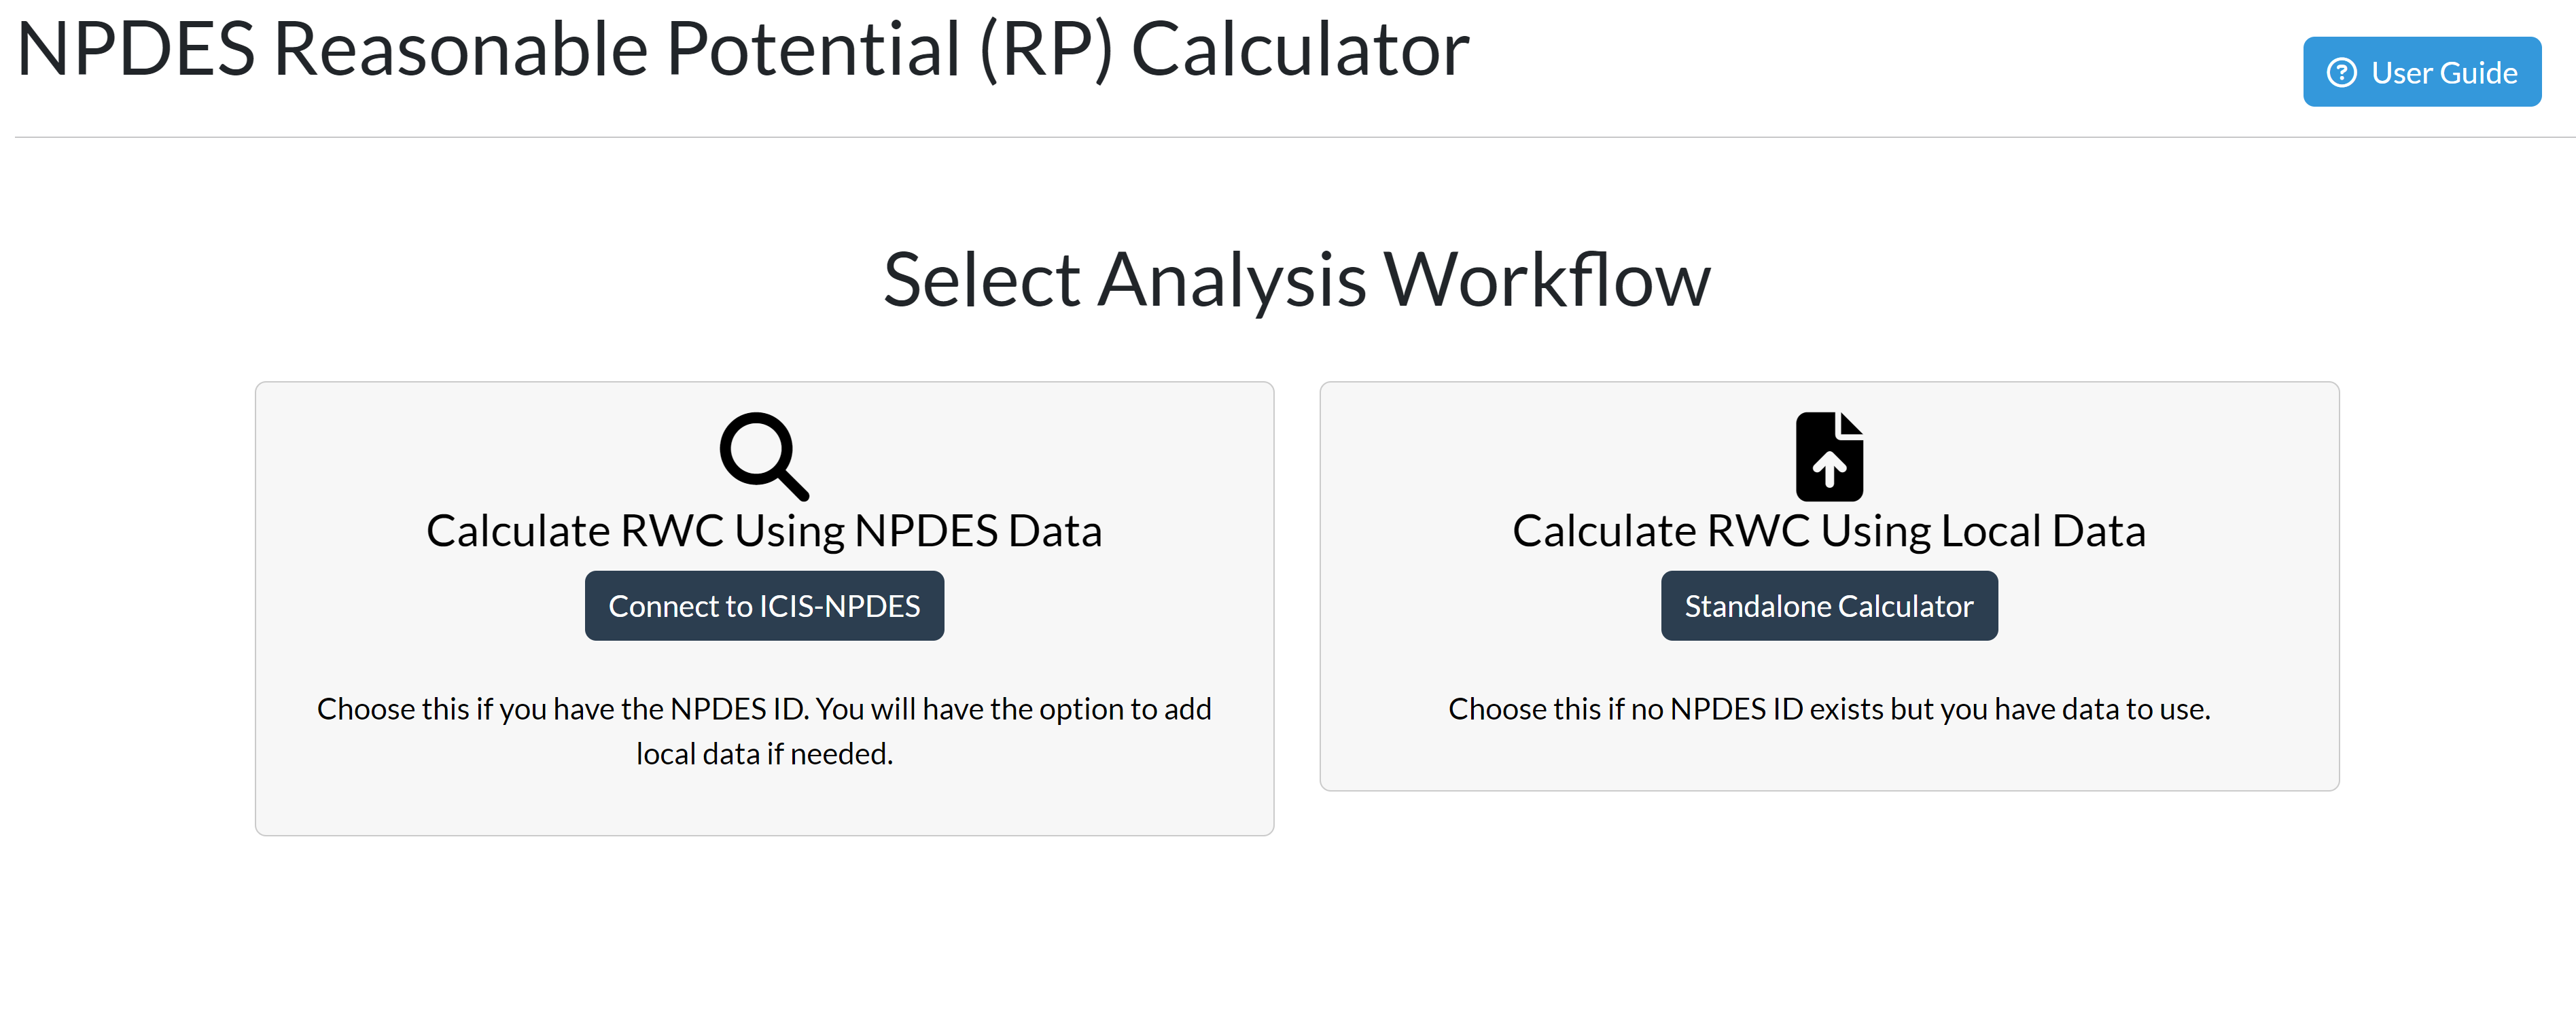
\includegraphics[keepaspectratio]{img/landing.png}}

}

\caption{Landing page with ``Connect to ICIS-NPDES'' and ``Standalone
Calculator'' workflow cards, and User Guide button in top right}

\end{figure}%

\begin{center}\rule{0.5\linewidth}{0.5pt}\end{center}

\section{NPDES Workflow}\label{sec-npdes-workflow}

Use this workflow when the facility has an active NPDES permit and
effluent monitoring data available in the local ICIS-NPDES database.

\subsection{Step 1: Search and Select a
Facility}\label{sec-select-facility}

Click \textbf{Connect to ICIS-NPDES} on the landing page. This opens the
facility selection page, which loads the list of NPDES permits for
Puerto Rico from the local ICIS-NPDES database at application startup.

Use the \textbf{Search Permit ID or Facility Name} box to find the
facility of interest. You can type either the NPDES ID (e.g.,
\texttt{PR0001031}) or any part of the facility name --- the search is
case-insensitive and matches partial strings. Select the facility from
the dropdown.

Once a facility is selected:

\begin{itemize}
\tightlist
\item
  The \textbf{map} displays a marker at the facility's reported
  latitude/longitude from the facility record in the local database
\item
  The \textbf{Facility Details} table displays key permit attributes
  from that facility record
\item
  The \textbf{Settings} panel and \textbf{Fetch DMR Data} button become
  visible
\end{itemize}

\begin{figure}[H]

{\centering \pandocbounded{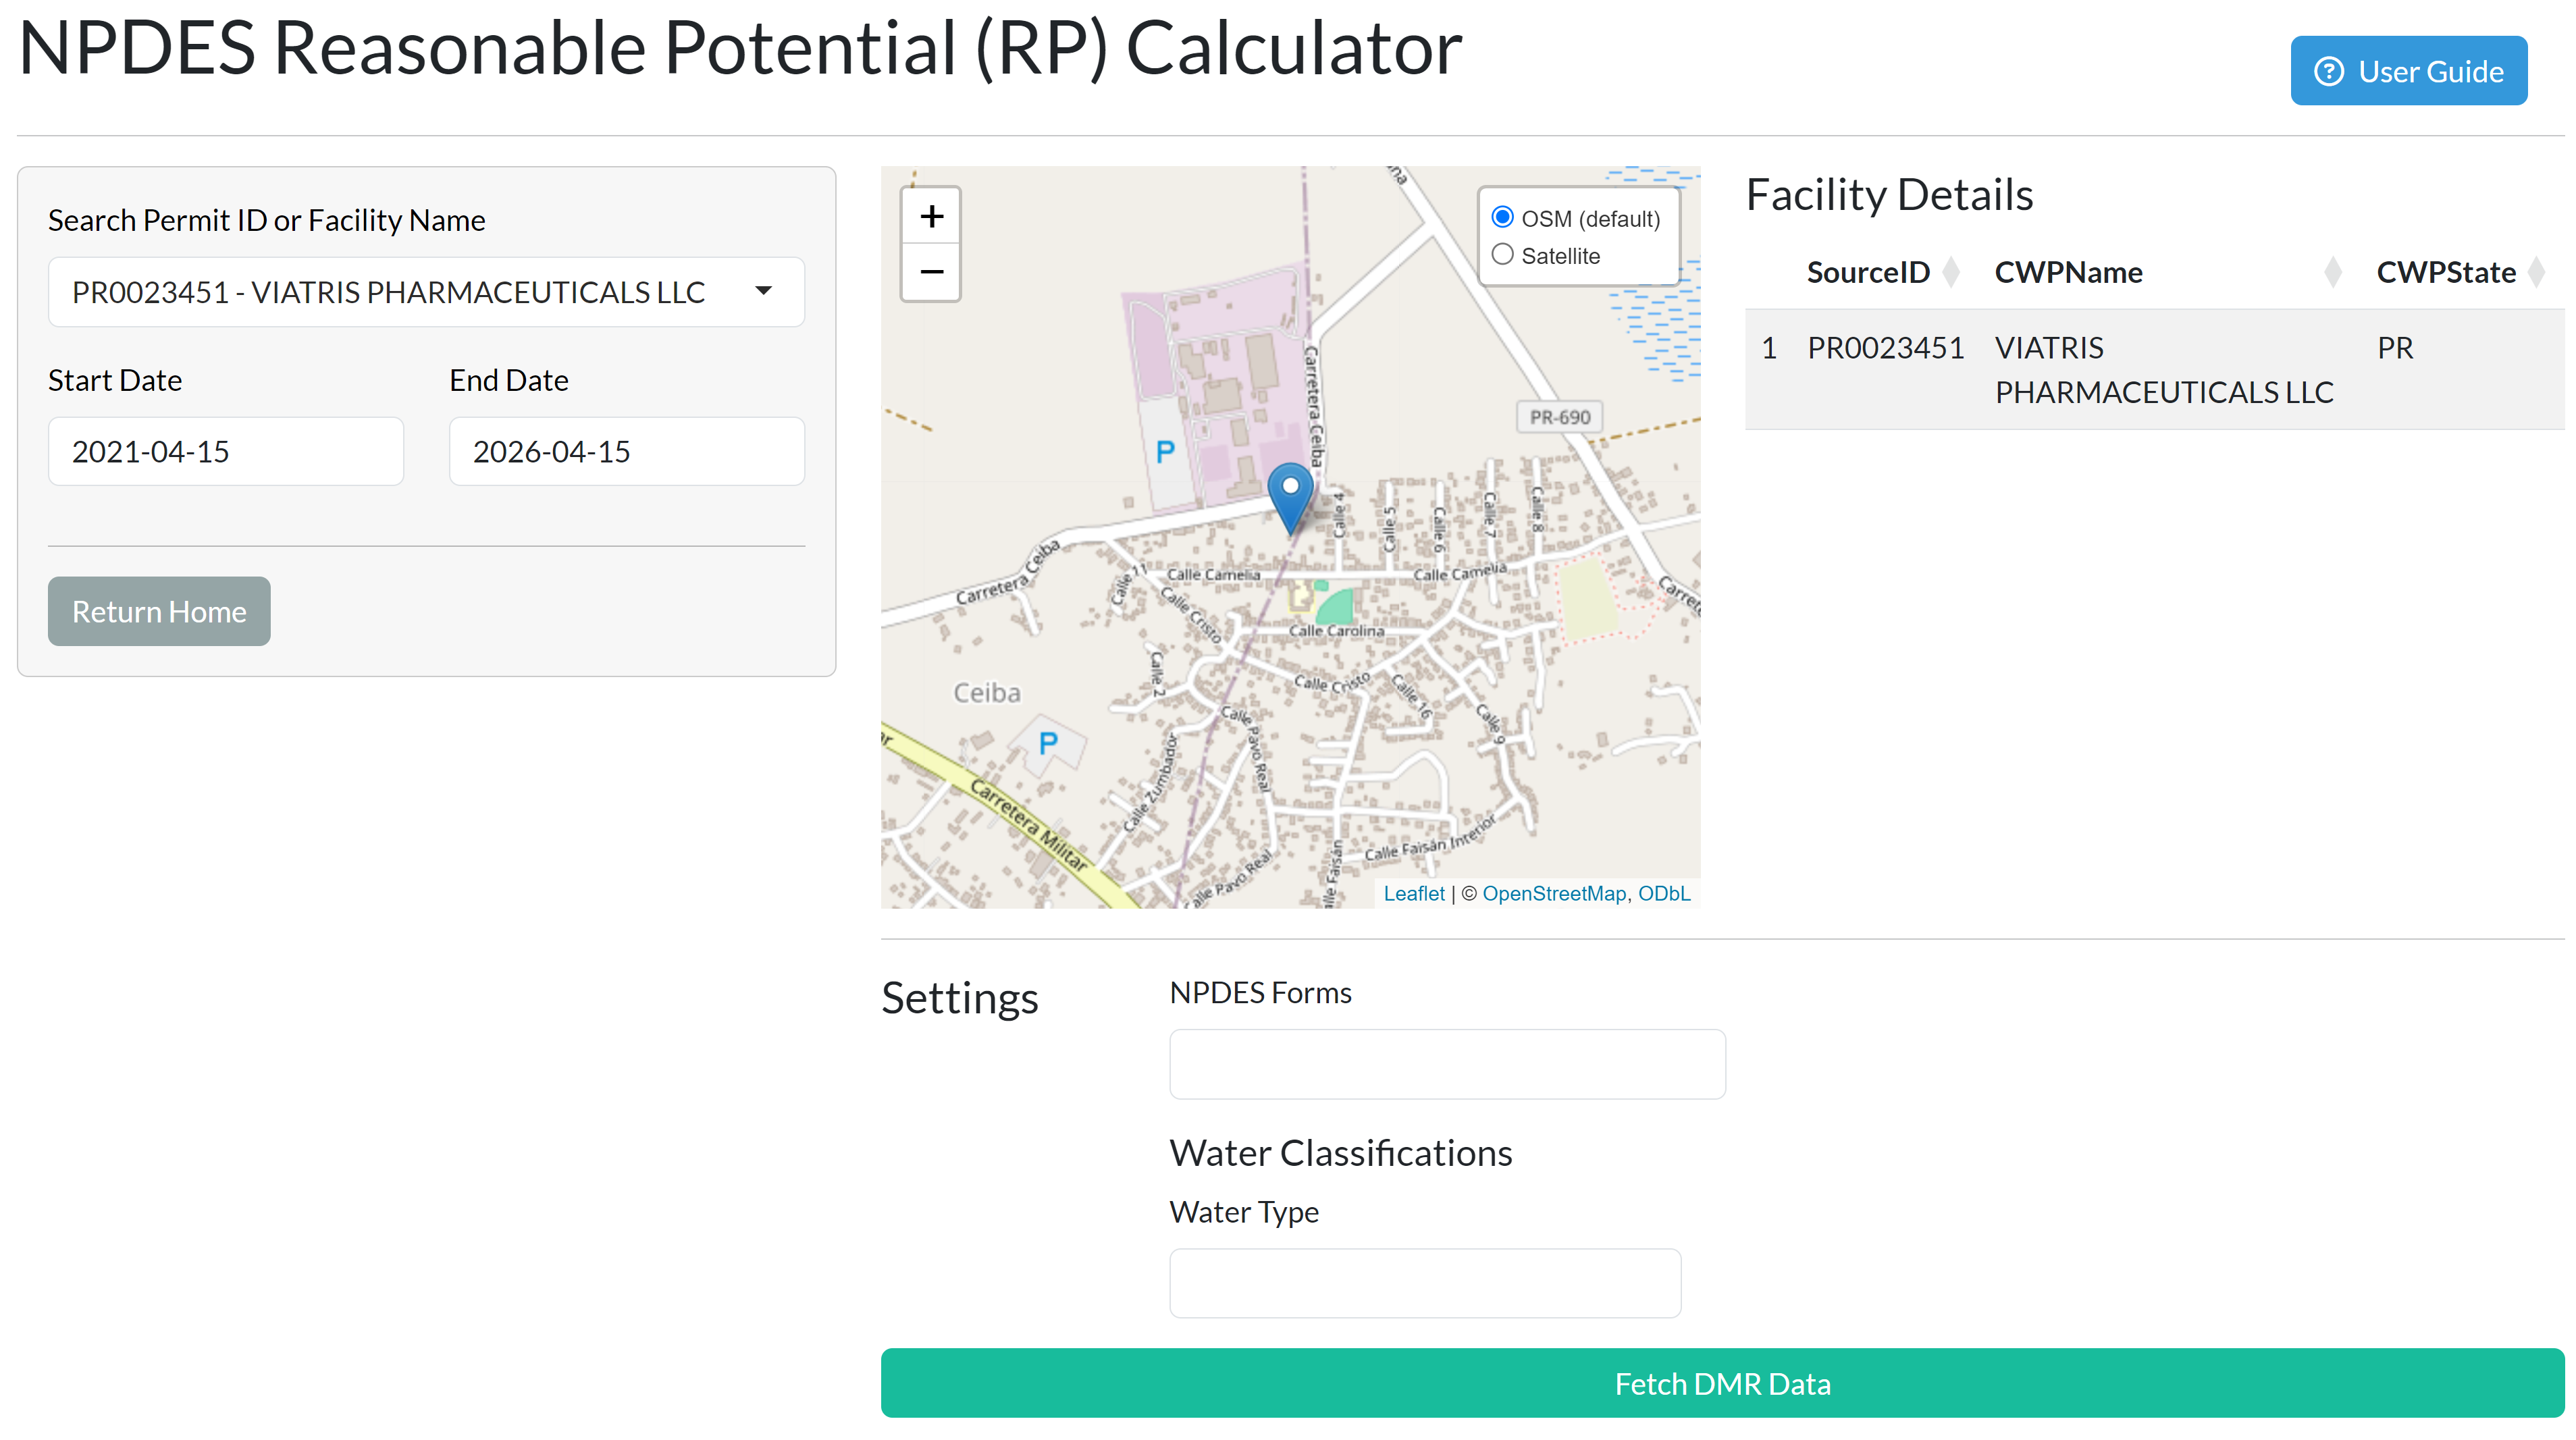
\includegraphics[keepaspectratio]{img/select_permit.png}}

}

\caption{Facility selection page showing the search box, map with
marker, and Facility Details table}

\end{figure}%

Set the \textbf{date range} for DMR retrieval using the Start Date and
End Date inputs. The default range is the five years prior to today's
date, which is appropriate for most permit reissuances. The date range
controls which DMR records are pulled from the database --- it does not
filter the facility list.

\begin{tcolorbox}[enhanced jigsaw, arc=.35mm, bottomrule=.15mm, bottomtitle=1mm, breakable, colback=white, colbacktitle=quarto-callout-note-color!10!white, colframe=quarto-callout-note-color-frame, coltitle=black, left=2mm, leftrule=.75mm, opacityback=0, opacitybacktitle=0.6, rightrule=.15mm, title=\textcolor{quarto-callout-note-color}{\faInfo}\hspace{0.5em}{Note}, titlerule=0mm, toprule=.15mm, toptitle=1mm]

\textbf{Selections persist within your session:} If you navigate away
from the search page and return --- for example, to revise a search ---
your permit ID, date range, NPDES forms, and water classification are
retained. These reset only when the app is restarted. Analysis Settings
on the Summary page (hardness, pH, temperature, dilution ratio,
confidence level) are not persisted, because they re-select naturally
when a different permit is fetched.

\end{tcolorbox}

\subsection{Step 2: Configure Filters}\label{sec-configure-filters}

Before fetching data, configure the two filters that control which
parameters are highlighted and which WQS criteria are in scope.

\subsubsection{NPDES Forms}\label{sec-npdes-forms}

Select one or more \textbf{NPDES application forms} from the
multi-select dropdown. NPDES applications require permittees to report
specific pollutants depending on the type of facility and the nature of
the discharge. The forms available in the app correspond to the standard
EPA application forms:

\begin{itemize}
\tightlist
\item
  \textbf{Form 2A} --- New and existing publicly owned treatment works
  (POTWs)
\item
  \textbf{Form 2B} --- Concentrated Animal Feeding Operations (CAFOs)
\item
  \textbf{Form 2C} --- Existing manufacturing, commercial, mining, and
  silviculture facilities
\item
  \textbf{Form 2D} --- New manufacturing, commercial, mining, and
  silviculture facilities
\item
  \textbf{Form 2E} --- Facilities that do not discharge process
  wastewater
\end{itemize}

The form selection defines the \textbf{universe of pollutants} expected
to be reported for the facility --- this determines which pollutants are
highlighted in the Data Overview (Coverage Summary) table, and it drives
the \emph{Reason Included} line in the report.

\begin{tcolorbox}[enhanced jigsaw, arc=.35mm, bottomrule=.15mm, bottomtitle=1mm, breakable, colback=white, colbacktitle=quarto-callout-important-color!10!white, colframe=quarto-callout-important-color-frame, coltitle=black, left=2mm, leftrule=.75mm, opacityback=0, opacitybacktitle=0.6, rightrule=.15mm, title=\textcolor{quarto-callout-important-color}{\faExclamation}\hspace{0.5em}{Important}, titlerule=0mm, toprule=.15mm, toptitle=1mm]

\textbf{Form selection is a display filter, not an analysis filter.}
Form selection no longer removes parameters from the calculation. Any
parameter that has DMR data and an applicable WQS criterion is evaluated
for RP regardless of its form association. Parameters not associated
with a selected form are labeled \emph{Not in selected forms} in the
Coverage Summary's Form column but are still included in the analysis.
This change prevents the old failure mode where a parameter with a real
criterion silently dropped out because it was not tied to the selected
form.

\end{tcolorbox}

\begin{tcolorbox}[enhanced jigsaw, arc=.35mm, bottomrule=.15mm, bottomtitle=1mm, breakable, colback=white, colbacktitle=quarto-callout-tip-color!10!white, colframe=quarto-callout-tip-color-frame, coltitle=black, left=2mm, leftrule=.75mm, opacityback=0, opacitybacktitle=0.6, rightrule=.15mm, title=\textcolor{quarto-callout-tip-color}{\faLightbulb}\hspace{0.5em}{Tip}, titlerule=0mm, toprule=.15mm, toptitle=1mm]

\textbf{Selecting the right form:} If you are unsure which form applies,
refer to the facility's permit application or its permit record. Most
municipal wastewater treatment plants use Form 2A. Most industrial and
manufacturing dischargers use Form 2C or 2D. When multiple forms apply
(e.g., a POTW receiving industrial pretreatment discharges), select all
applicable forms.

\end{tcolorbox}

\subsubsection{Water Classifications}\label{sec-water-type-filter}

Select one or more \textbf{water classifications} from the multi-select
dropdown. The choices correspond to Puerto Rico's PRWQSR classifications
described in Section~\ref{sec-classifications}:

{\def\LTcaptype{none} % do not increment counter
\begin{longtable}[]{@{}
  >{\raggedright\arraybackslash}p{(\linewidth - 2\tabcolsep) * \real{0.5000}}
  >{\raggedright\arraybackslash}p{(\linewidth - 2\tabcolsep) * \real{0.5000}}@{}}
\toprule\noalign{}
\begin{minipage}[b]{\linewidth}\raggedright
Selection
\end{minipage} & \begin{minipage}[b]{\linewidth}\raggedright
Maps to PRWQSR Classification
\end{minipage} \\
\midrule\noalign{}
\endhead
\bottomrule\noalign{}
\endlastfoot
All & All classes in the crosswalk \\
Class SB & Class SB coastal and estuarine waters \\
Class SD & Class SD surface waters (including drinking water
subclass) \\
Class SG & Class SG ground waters \\
Surface Waters & General surface water standards (Rule 1303.1) \\
\end{longtable}
}

These selections determine which WQS criteria rows are active for
comparison. When multiple classifications are selected, the app performs
the RP comparison independently for each class and reports the
worst-case result. Select \textbf{All} to evaluate against every
applicable standard in the crosswalk --- appropriate when the receiving
water classification is uncertain or when you want to be comprehensive.

\begin{tcolorbox}[enhanced jigsaw, arc=.35mm, bottomrule=.15mm, bottomtitle=1mm, breakable, colback=white, colbacktitle=quarto-callout-important-color!10!white, colframe=quarto-callout-important-color-frame, coltitle=black, left=2mm, leftrule=.75mm, opacityback=0, opacitybacktitle=0.6, rightrule=.15mm, title=\textcolor{quarto-callout-important-color}{\faExclamation}\hspace{0.5em}{Important}, titlerule=0mm, toprule=.15mm, toptitle=1mm]

\textbf{Class SD and conditional criteria:} If \textbf{Class SD} is
selected, the conditional receiving water inputs panel appears (see
Section~\ref{sec-hardness-settings}). You will need to provide a
hardness value or choose the range analysis option, and pH and
temperature for TAN, before running RP. This panel is only shown for
Class SD because the hardness-dependent metal criteria and the TAN
criterion are specific to Class SD surface waters under the PRWQSR.

\end{tcolorbox}

\subsection{Step 3: Fetch DMR Data}\label{sec-fetch-dmr}

Click \textbf{Fetch DMR Data}. The app queries the local ICIS-NPDES
database for effluent monitoring records matching the selected permit ID
and date range, then applies the following processing steps
automatically:

\textbf{Statistic tagging:} Each DMR record is tagged with a semantic
statistic token (daily maximum, daily minimum, geometric mean, 90th
percentile, or average) derived from its ICIS statistical-base code.
This is what lets the app keep the right records for each criterion ---
the minimum for a floor parameter, the geometric mean for a bacteria
criterion --- instead of keeping only maximums. A parameter with data
but no matching criterion is retained rather than discarded, so it can
be surfaced on the Needs Attention tab (see
Section~\ref{sec-needs-attention}) rather than vanishing silently.

\textbf{NODI code handling:} Records with NODI codes B (``no
discharge'') or Q (``no discharge this period'') are set to a value of
zero. This is consistent with the approach in the TSD --- a period of no
discharge represents a zero concentration and should be included in the
sample set. Records with other NODI codes that prevent a numeric value
from being reported are excluded.

\textbf{Unit detection and filling:} DMR reports occasionally omit unit
labels for individual records, particularly for NODI-coded rows. The app
fills missing units by using the most frequently reported unit for that
parameter across the permit's records, falling back to the WQS unit hint
from the crosswalk if all records for the parameter have missing units.

\textbf{Unit conversion:} Each reported value is checked against the WQS
unit for its parameter. The converter handles concentration conversions
(µg/L ↔ mg/L, ng/L → µg/L or mg/L, ppm → mg/L or µg/L), recognizes
several units that are written differently but mean the same thing
(e.g., ICIS long-form bacteria and color units), and converts Fahrenheit
to Celsius for temperature. Mass-load and flow units (e.g., kg/day, MGD)
are \textbf{excluded} from the WQS comparison by design rather than
treated as errors, because a load cannot be compared to a concentration
criterion. When a parameter has no WQS criterion for the selected water
class, its records are flagged \textbf{NO WQS}. A genuinely unrecognized
unit is flagged \textbf{FAIL} and the value is retained at face value.
Every status is shown in the Coverage Summary and carried into the
report (see Section~\ref{sec-data-overview}).

After a successful fetch, the app navigates to the \textbf{Summary (Data
Overview) page}.

\subsection{Step 4: Review the Data Overview}\label{sec-data-overview}

The Data Overview page displays the \textbf{Coverage Summary} table,
which lists the pollutants relevant to this analysis --- those
associated with the selected NPDES forms plus any additional parameters
that have DMR data --- alongside a count of available DMR samples and a
unit conversion status indicator. Parameters not associated with a
selected form are marked \emph{Not in selected forms} in the Form
column.

\begin{figure}[H]

{\centering \pandocbounded{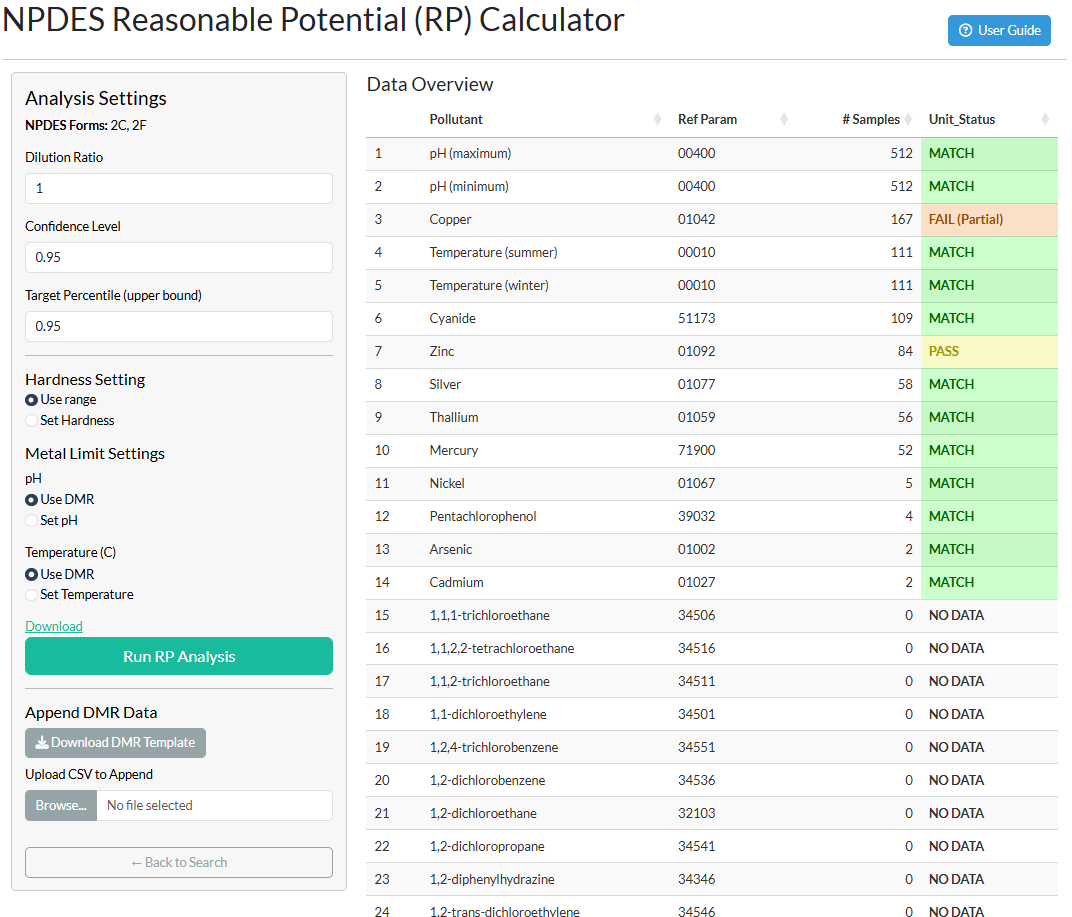
\includegraphics[keepaspectratio]{img/review.png}}

}

\caption{Summary page showing the Coverage Summary table with unit
status column}

\end{figure}%

\textbf{Understanding the Coverage Summary columns:}

{\def\LTcaptype{none} % do not increment counter
\begin{longtable}[]{@{}
  >{\raggedright\arraybackslash}p{(\linewidth - 2\tabcolsep) * \real{0.5000}}
  >{\raggedright\arraybackslash}p{(\linewidth - 2\tabcolsep) * \real{0.5000}}@{}}
\toprule\noalign{}
\begin{minipage}[b]{\linewidth}\raggedright
Column
\end{minipage} & \begin{minipage}[b]{\linewidth}\raggedright
Description
\end{minipage} \\
\midrule\noalign{}
\endhead
\bottomrule\noalign{}
\endlastfoot
Pollutant & NPDES pollutant name from the form crosswalk \\
Form & The NPDES application form(s) that require this pollutant, or
\emph{Not in selected forms} \\
Ref Param & The DMR parameter code(s) matched to this pollutant in the
crosswalk \\
\# Samples & Count of qualifying DMR records retrieved for this permit
and date range \\
Unit Status & Result of the unit conversion check (see below) \\
\end{longtable}
}

\textbf{Unit Status values:}

{\def\LTcaptype{none} % do not increment counter
\begin{longtable}[]{@{}
  >{\raggedright\arraybackslash}p{(\linewidth - 4\tabcolsep) * \real{0.3333}}
  >{\raggedright\arraybackslash}p{(\linewidth - 4\tabcolsep) * \real{0.3333}}
  >{\raggedright\arraybackslash}p{(\linewidth - 4\tabcolsep) * \real{0.3333}}@{}}
\toprule\noalign{}
\begin{minipage}[b]{\linewidth}\raggedright
Status
\end{minipage} & \begin{minipage}[b]{\linewidth}\raggedright
Meaning
\end{minipage} & \begin{minipage}[b]{\linewidth}\raggedright
Action
\end{minipage} \\
\midrule\noalign{}
\endhead
\bottomrule\noalign{}
\endlastfoot
MATCH & Reported units already match the WQS unit (including recognized
aliases) --- no conversion needed & None required \\
PASS & Units differed but a multiplicative or temperature conversion was
successfully applied & Conversion is shown in the report \\
FAIL (Partial) & Some eligible records converted successfully but others
could not & Proceed with caution; non-convertible records are dropped
from the RP calculation \\
FAIL & No eligible record could be converted to the WQS unit
(unrecognized unit) & Investigate the DMR data; values are retained at
face value but dropped from RP \\
EXCLUDED & Every record is a mass-load or flow unit (e.g., kg/day, MGD)
& Informational --- these cannot be compared to a concentration
criterion and are excluded by design \\
NO WQS & No WQS criterion exists for this parameter in the selected
water class & Informational --- see the \textbf{Needs Attention} tab to
add a manual criterion if appropriate \\
NO DATA & Parameter is in the crosswalk but had no DMR records &
Informational --- nothing to evaluate \\
\end{longtable}
}

EXCLUDED, NO WQS, and NO DATA are informational, not errors, and are
color-coded distinctly (grey / blue-grey / light-grey) from the FAIL
states (red / orange). A FAIL or FAIL (Partial) status does not prevent
the analysis from running, but it means that some or all values for that
parameter may be in the wrong units. Before proceeding, verify the DMR
data in the source ICIS-NPDES record for any parameters showing a FAIL
status --- the issue is often a data entry error in the original
submission.

\subsection{Step 4b: Resolve Parameters Needing
Attention}\label{sec-needs-attention}

The Summary page has three tabs: \textbf{Data Overview} (the Coverage
Summary described above), \textbf{⚠ Needs Attention}, and \textbf{WQS
Reference}.

The \textbf{Needs Attention} tab lists any parameter that has DMR data
but no usable WQS criterion for the selected water class. Each flagged
parameter is shown in an orange-bordered card with the reason it was
flagged:

\begin{itemize}
\tightlist
\item
  \textbf{Wrong water class} --- a WQS criterion exists for this
  parameter, but not for the class(es) you selected.
\item
  \textbf{No crosswalk entry} --- the parameter code has no WQS entry at
  all.
\item
  \textbf{Missing criterion value} --- a crosswalk entry exists but its
  value is blank.
\item
  \textbf{Reported statistic does not match criterion} --- the parameter
  matches a criterion, but its DMR data reports only a statistic the
  criterion is not written against (for example, a daily maximum
  reported against a geometric-mean criterion). This is a matched code,
  so it is added to the flagged set rather than dropped.
\end{itemize}

For each flagged parameter you choose \textbf{Include with manual WQS}
or \textbf{Exclude from analysis} using the radio buttons. To include a
parameter, fill in the manual-entry fields: a \textbf{Criterion Value},
a \textbf{Unit} (limited to units the converter can handle), a
\textbf{Criterion Type} (e.g., \emph{Aquatic Life -- Acute}), a
\textbf{Criterion Direction}, the \textbf{Water Class(es)} it applies
to, and a required \textbf{Basis / Notes} field. To exclude a parameter,
provide a required reason. Included parameters are injected as manual
criteria when you run the analysis; excluded parameters are recorded in
the report's \emph{Excluded Parameters} section for the permanent
record.

\begin{tcolorbox}[enhanced jigsaw, arc=.35mm, bottomrule=.15mm, bottomtitle=1mm, breakable, colback=white, colbacktitle=quarto-callout-note-color!10!white, colframe=quarto-callout-note-color-frame, coltitle=black, left=2mm, leftrule=.75mm, opacityback=0, opacitybacktitle=0.6, rightrule=.15mm, title=\textcolor{quarto-callout-note-color}{\faInfo}\hspace{0.5em}{Note}, titlerule=0mm, toprule=.15mm, toptitle=1mm]

\textbf{Criterion Direction --- ceiling vs floor.} The direction
selector offers \emph{Ceiling --- shall not exceed (\textgreater)} and
\emph{Floor --- shall not fall below (\textless)}. This matters because
a hand-entered floor standard (a dissolved-oxygen-style minimum) would
otherwise be treated as a ceiling and projected incorrectly. A floor
entry is evaluated by direct comparison against the observed
\textbf{minimum}, and a value exactly on the criterion is treated as
compliant (the comparison is a strict inequality). Known parameters
re-added by hand inherit their built-in profile --- a direct parameter
stays direct --- so the direction selector governs genuinely new
parameters.

\end{tcolorbox}

\begin{tcolorbox}[enhanced jigsaw, arc=.35mm, bottomrule=.15mm, bottomtitle=1mm, breakable, colback=white, colbacktitle=quarto-callout-note-color!10!white, colframe=quarto-callout-note-color-frame, coltitle=black, left=2mm, leftrule=.75mm, opacityback=0, opacitybacktitle=0.6, rightrule=.15mm, title=\textcolor{quarto-callout-note-color}{\faInfo}\hspace{0.5em}{Note}, titlerule=0mm, toprule=.15mm, toptitle=1mm]

\textbf{Green alias hints.} Some cards show a green \textbf{Hint}
pointing to the code and value that applies --- for example, when the
criterion for an analyte lives under a synonym parameter code that
differs from the one the permittee reported. The hint tells you which
criterion ID and value to enter rather than making you hunt for it. Use
the \textbf{WQS Reference} tab --- a read-only, searchable view of the
full crosswalk --- to confirm criterion IDs and values before entering a
manual criterion.

\end{tcolorbox}

\begin{tcolorbox}[enhanced jigsaw, arc=.35mm, bottomrule=.15mm, bottomtitle=1mm, breakable, colback=white, colbacktitle=quarto-callout-important-color!10!white, colframe=quarto-callout-important-color-frame, coltitle=black, left=2mm, leftrule=.75mm, opacityback=0, opacitybacktitle=0.6, rightrule=.15mm, title=\textcolor{quarto-callout-important-color}{\faExclamation}\hspace{0.5em}{Important}, titlerule=0mm, toprule=.15mm, toptitle=1mm]

\textbf{Run RP is gated on resolution.} The \textbf{Run RP Analysis}
button stays disabled until every flagged parameter has an
Include/Exclude decision. If you need to proceed without resolving them,
use the red \textbf{⚡ Quick Run (Drop Unresolved)} button --- it
auto-excludes all unresolved parameters and stamps a prominent
``preliminary report'' warning on the generated report so the omission
is on the permanent record.

\end{tcolorbox}

Parameters that don't require resolution are never flagged:
hardness-dependent metals and TAN (whose criteria are computed at run
time from your hardness, pH, and temperature inputs) are treated as
matched, and parameters reported only in mass-load or flow units are
dropped from the flag pass because they can never be compared to a
concentration criterion.

\begin{figure}[H]

{\centering \pandocbounded{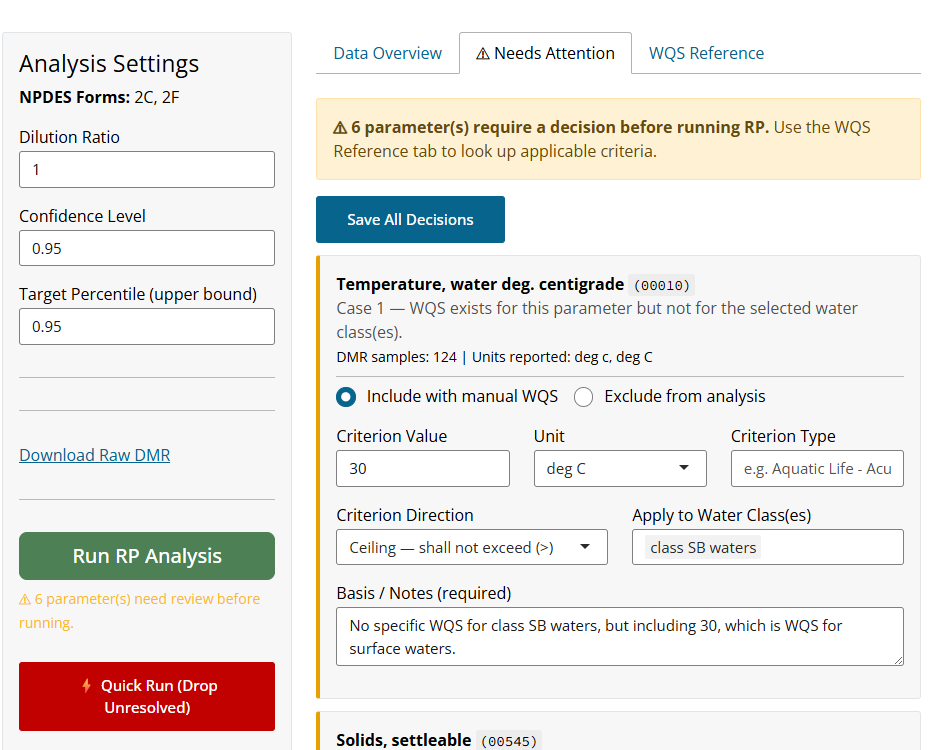
\includegraphics[keepaspectratio]{img/needs_attention.png}}

}

\caption{The Needs Attention tab with a flagged parameter expanded,
showing the Include/Exclude radio, Criterion Direction dropdown,
manual-entry fields, and a green code-alias Hint}

\end{figure}%

\subsection{Step 5: Configure Analysis
Settings}\label{sec-analysis-settings}

The left panel of the Summary page contains the Analysis Settings. These
control the statistical and receiving water parameters used in the RWC
and RP calculations. A full description of the methodology behind each
setting is provided in Section~\ref{sec-methodology}.

\subsubsection{Dilution Ratio}\label{sec-dilution-ratio}

The \textbf{Dilution Ratio} (DR) is the ratio of the total flow at the
edge of the mixing zone (effluent plus receiving water) to the effluent
flow alone. It represents the degree to which the discharge is diluted
by the receiving water at the point of compliance. The default value is
1, which means no dilution is assumed --- the effluent concentration
itself is compared to the WQS criterion. This is the conservative
default and is appropriate when:

\begin{itemize}
\tightlist
\item
  No mixing zone has been authorized
\item
  Dilution data are unavailable
\item
  The receiving water is intermittent or has negligible flow relative to
  the discharge
\end{itemize}

If a mixing zone authorization exists or a dilution analysis has been
performed, enter the appropriate dilution ratio here. Values greater
than 1 reduce the RWC and make an RP finding less likely. The dilution
ratio applies only to projected criteria; direct-comparison parameters
(Section~\ref{sec-direct}) do not use it. The dilution ratio is captured
in the report.

\begin{tcolorbox}[enhanced jigsaw, arc=.35mm, bottomrule=.15mm, bottomtitle=1mm, breakable, colback=white, colbacktitle=quarto-callout-warning-color!10!white, colframe=quarto-callout-warning-color-frame, coltitle=black, left=2mm, leftrule=.75mm, opacityback=0, opacitybacktitle=0.6, rightrule=.15mm, title=\textcolor{quarto-callout-warning-color}{\faExclamationTriangle}\hspace{0.5em}{Warning}, titlerule=0mm, toprule=.15mm, toptitle=1mm]

\textbf{Dilution ratio and mixing zones:} A dilution ratio greater than
1 implies that a mixing zone exists. Ensure that any mixing zone used
here is either already authorized by DNER under Rule 1305 of the PRWQSR,
or that you have an appropriate basis for the dilution value. Using an
unsupported dilution ratio in the RP analysis may underestimate RP and
result in a permit that does not adequately protect water quality.

\end{tcolorbox}

\subsubsection{Confidence Level and Target
Percentile}\label{sec-cl-percentile}

These two parameters control the statistical projection used to compute
the Multiplying Factor (MF) --- see Section~\ref{sec-mf} for a full
explanation.

\textbf{Confidence Level (CL):} The probability (a proportion between 0
and 1) that the highest observed value in the sample set exceeds the
stated percentile of the underlying effluent distribution. The default
is 0.95 (95\%). EPA's TSD presents lookup tables at both 95\% and 99\%
confidence levels; the 95\% level is the default used in most regional
RP guidance.

\textbf{Target Percentile:} The upper bound of the effluent distribution
that the projected RWC is designed to represent, expressed as a
proportion. The default is 0.95 (95th percentile). Together with the
confidence level, this defines how conservatively the projection treats
variability in the effluent --- a higher target percentile produces a
larger MF and a more conservative RP determination.

\begin{tcolorbox}[enhanced jigsaw, arc=.35mm, bottomrule=.15mm, bottomtitle=1mm, breakable, colback=white, colbacktitle=quarto-callout-note-color!10!white, colframe=quarto-callout-note-color-frame, coltitle=black, left=2mm, leftrule=.75mm, opacityback=0, opacitybacktitle=0.6, rightrule=.15mm, title=\textcolor{quarto-callout-note-color}{\faInfo}\hspace{0.5em}{Note}, titlerule=0mm, toprule=.15mm, toptitle=1mm]

\textbf{Default settings:} The defaults of 95\% confidence level and
95th percentile target are consistent with EPA Region 2 guidance for RP
determinations using existing DMR data. If regional or program-specific
guidance specifies different values (e.g., 99\%/99\% for certain
pollutant categories), adjust these settings accordingly. The values
used are documented in the report.

\end{tcolorbox}

\subsubsection{Hardness Settings (Class SD
only)}\label{sec-hardness-settings}

This panel appears only when \textbf{Class SD} is selected as a water
classification. It controls how the app handles the seven
hardness-dependent metal criteria in the PRWQSR (see
Section~\ref{sec-metals}).

\textbf{Hardness value (mg/L as CaCO₃):} Enter a numeric hardness value
for the receiving water if a measured or estimated value is available.
The app uses this value to compute the metal criterion from the hardness
regression equations in Rule 1303.1(J)(1) and uses it directly in the RP
comparison. The default is 100 mg/L as CaCO₃, a reasonable midrange
value for Puerto Rico surface waters in the absence of site-specific
data; use a measured value whenever possible. If no single hardness is
appropriate, the range analysis option reports the criterion as a
\textbf{DEPENDS} result with a critical-hardness annotation (see
Section~\ref{sec-interpret-depends}).

\subsubsection{pH and Temperature (for TAN, Class SD
only)}\label{sec-ph-temp-settings}

These inputs appear within the Class SD conditional panel and are used
for the Total Ammonia Nitrogen (TAN) RP evaluation (see
Section~\ref{sec-tan}). The TAN criterion under Rule 1303.2(C)(2)(l) is
a function of receiving water pH and temperature.

\textbf{Use DMR data:} If pH (parameter code 00400) and temperature
(parameter code 00010) data are available in the DMR records, the app
uses those values to compute a time-varying TAN limit --- one for each
monitoring period that has both a pH and temperature record. The RP
determination for TAN is YES if the TAN RWC exceeds the criterion at any
point in the monitoring record (the ``ever crossed'' rule). The mean TAN
limit is shown in summary tables and plots for display purposes.

\textbf{Override with fixed values:} If the DMR does not include pH or
temperature, or if you prefer to use design receiving water conditions,
enter fixed pH and temperature values. The app uses these constant
values to compute a single TAN limit for comparison against the TAN RWC.

\textbf{Receiving Water pH (SU):} Valid range 0--14. Default is 6.0 SU,
which represents a slightly acidic condition and produces a more
conservative (lower) TAN criterion. For context, Class SD waters have a
pH standard of 6.0--9.0 SU (Rule 1303.2(C)(2)(d)).

\textbf{Receiving Water Temperature (°C):} Valid range 0--50 °C. Default
is 30 °C, consistent with Puerto Rico's thermal discharge standard of 30
°C (Rule 1303.1(D)(1)).

\subsection{Step 6: Append Local DMR Data
(Optional)}\label{sec-append-dmr}

If you have effluent monitoring data that are not in the database ---
for example, data from a recent sampling event not yet submitted to EPA,
or data from a non-standard monitoring program --- you can append those
records to the retrieved dataset before running the RP analysis.

\textbf{Download the DMR Template:} Click \textbf{Download DMR Template}
to download a CSV file pre-populated with the parameter codes and
expected WQS units for the selected facility and forms. The template
includes one row per parameter code with blank value fields.

\textbf{Complete the template:} Fill in the following columns for each
record you want to add:

{\def\LTcaptype{none} % do not increment counter
\begin{longtable}[]{@{}
  >{\raggedright\arraybackslash}p{(\linewidth - 2\tabcolsep) * \real{0.5000}}
  >{\raggedright\arraybackslash}p{(\linewidth - 2\tabcolsep) * \real{0.5000}}@{}}
\toprule\noalign{}
\begin{minipage}[b]{\linewidth}\raggedright
Column
\end{minipage} & \begin{minipage}[b]{\linewidth}\raggedright
Description
\end{minipage} \\
\midrule\noalign{}
\endhead
\bottomrule\noalign{}
\endlastfoot
\texttt{parameter\_code} & 5-digit DMR parameter code (pre-filled from
crosswalk) \\
\texttt{parameter\_desc} & Parameter description (informational only) \\
\texttt{dmr\_value\_nmbr} & Observed concentration (numeric) \\
\texttt{dmr\_unit\_desc} & Units for the reported value \\
\texttt{monitoring\_period\_end\_date} & End date of the monitoring
period (\texttt{YYYY-MM-DD} or \texttt{MM/DD/YYYY}) \\
\texttt{perm\_feature\_nmbr} & Outfall identifier (e.g.,
\texttt{001}) \\
\end{longtable}
}

Multiple rows can be added for a single parameter code --- add one row
per monitoring period per outfall. Save the file as a CSV.

\textbf{Upload the completed template:} Click \textbf{Upload CSV to
Append} and select your completed file. The app validates the required
columns, attempts unit conversion, and appends the records to the
existing DMR dataset. A notification confirms the number of rows added.

\begin{tcolorbox}[enhanced jigsaw, arc=.35mm, bottomrule=.15mm, bottomtitle=1mm, breakable, colback=white, colbacktitle=quarto-callout-warning-color!10!white, colframe=quarto-callout-warning-color-frame, coltitle=black, left=2mm, leftrule=.75mm, opacityback=0, opacitybacktitle=0.6, rightrule=.15mm, title=\textcolor{quarto-callout-warning-color}{\faExclamationTriangle}\hspace{0.5em}{Warning}, titlerule=0mm, toprule=.15mm, toptitle=1mm]

\textbf{Unit responsibility:} When appending local data, you are
responsible for ensuring that the units in \texttt{dmr\_unit\_desc}
match what was actually measured. The app will attempt to convert to WQS
units, but if the reported unit is not recognized, the value is retained
at face value and flagged with a FAIL conversion status. Unit mismatches
in appended data appear in the Coverage Summary table.

\end{tcolorbox}

\subsection{Step 7: Run the RP Analysis}\label{sec-run-rp}

Click \textbf{Run RP Analysis}. (This button is enabled once every
flagged parameter has been resolved --- see
Section~\ref{sec-needs-attention}.) The app computes the RP
determination for every parameter × outfall combination in the dataset
using the settings configured in Step 5: projected criteria run through
the RWC calculation, and direct-comparison criteria are tested against
the appropriate observed statistic. When the calculation is complete,
the app navigates to the \textbf{Findings page}.

\begin{center}\rule{0.5\linewidth}{0.5pt}\end{center}

\section{Standalone Workflow}\label{sec-standalone-workflow}

Use the Standalone Calculator when no NPDES ID exists (e.g., for a new
permit application) or when you have local monitoring data and prefer
not to retrieve data from the database.

Click \textbf{Standalone Calculator} on the landing page. Download the
DMR template, complete it with your monitoring data (the same columns
described in Section~\ref{sec-append-dmr}), and upload it. Because
standalone uploads have no ICIS statistical-base codes, every uploaded
record is treated as a daily maximum unless the criterion it matches
requires a different statistic; where a criterion needs a statistic your
upload does not carry, the parameter is surfaced on the Needs Attention
tab. From the upload onward, the Standalone workflow uses the same
Analysis Settings, Findings, and Report pages as the NPDES workflow.

\begin{center}\rule{0.5\linewidth}{0.5pt}\end{center}

\section{The Findings Page}\label{sec-findings}

After running the analysis, the Findings page presents the results. The
left sidebar lets you select an \textbf{Outfall} and a
\textbf{Parameter/Pollutant}, shows the \textbf{Quick Stats} panel for
the current selection, and provides the \textbf{Download Report} button
and \textbf{Include Data in Download} checkbox. Internal outfalls are
shown in bold red in the selector and throughout the page so they are
not mistaken for external outfalls.

\begin{figure}[H]

{\centering \pandocbounded{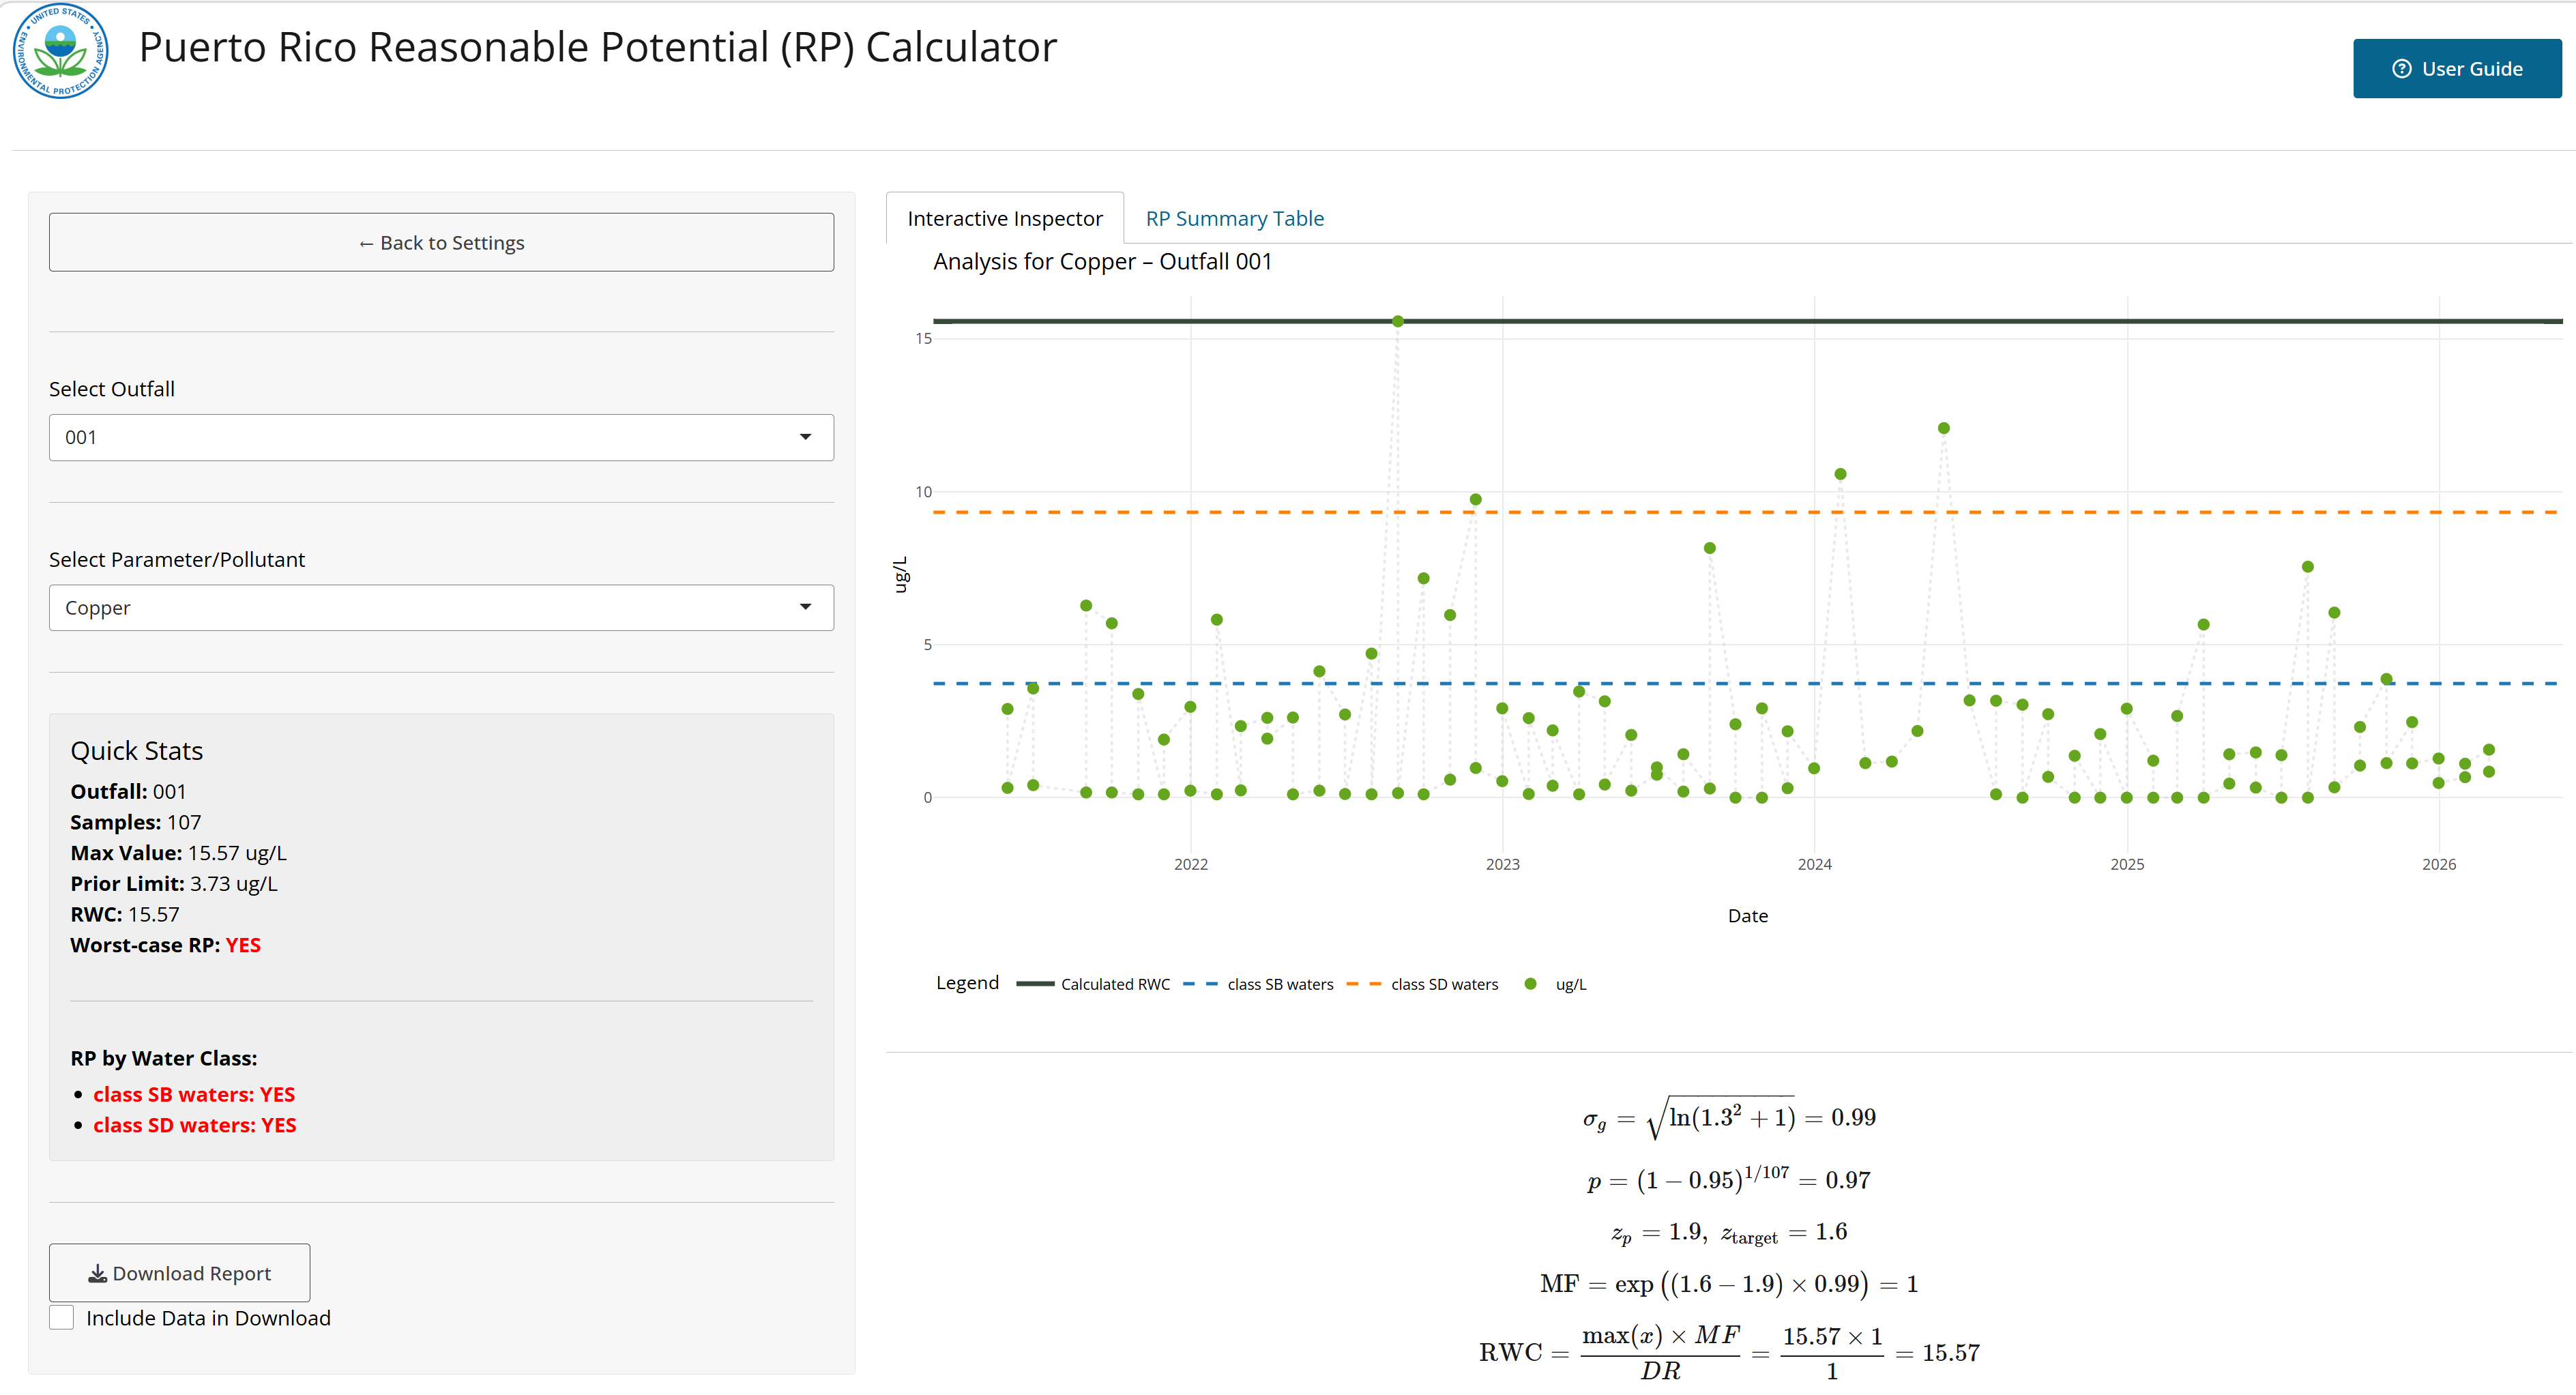
\includegraphics[keepaspectratio]{img/findings.png}}

}

\caption{Findings page overview showing sidebar with outfall/pollutant
selectors and Quick Stats panel, and main tabbed plot area}

\end{figure}%

The main panel has two tabs: the \textbf{Interactive Inspector} (a plot
plus a math inspector that shows the step-by-step calculation) and the
\textbf{RP Summary Table}.

\subsection{Quick Stats}\label{sec-quick-stats}

The Quick Stats panel summarizes the selected outfall × pollutant. It
shows the outfall, the sample count, the assessed value, any prior
permit limit, the worst-case RP, and --- when present --- a
criterion-specific note carried from the crosswalk.

\begin{figure}[H]

{\centering 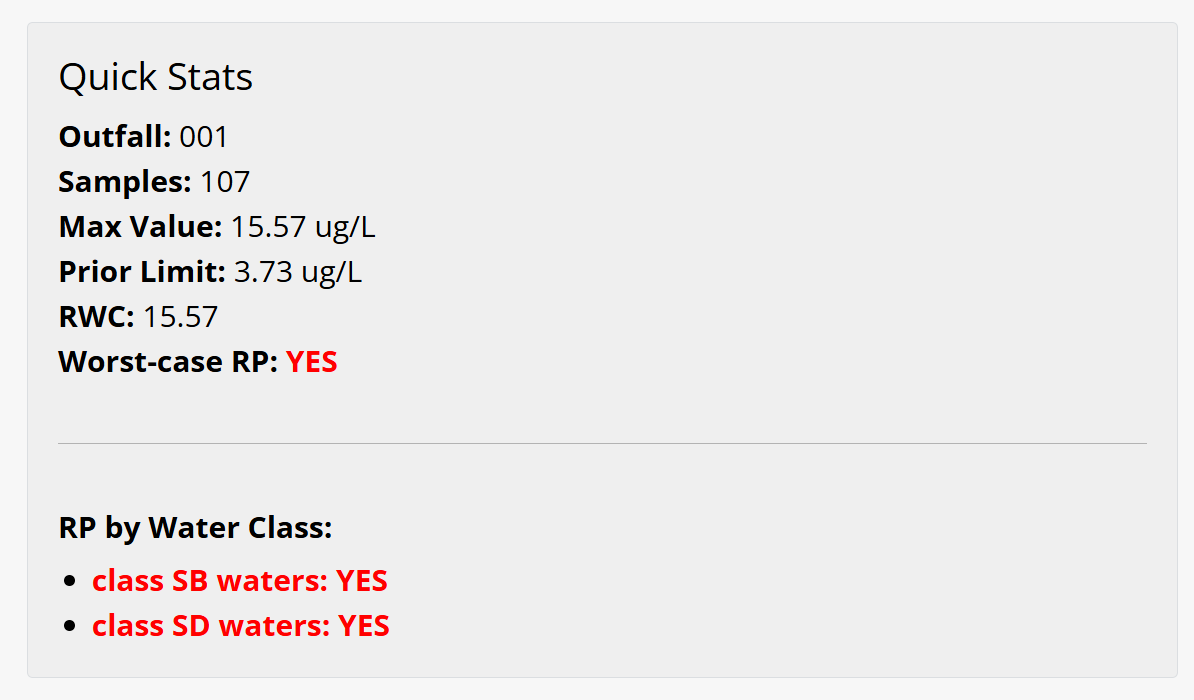
\includegraphics[width=0.5\linewidth,height=\textheight,keepaspectratio]{img/quick_stats.png}

}

\caption{Quick Stats panel showing Worst-case RP highlighted in red
(YES), with per-class breakdown}

\end{figure}%

A few fields adapt to the type of criterion:

\begin{itemize}
\tightlist
\item
  \textbf{Max Value / Min Value.} For ceiling criteria the panel shows
  the observed maximum; for floor criteria (dissolved oxygen, pH
  minimum) it shows the observed minimum, because the minimum is the
  compliance-relevant statistic.
\item
  \textbf{RWC vs.~Observed value.} For projected criteria the panel
  shows the calculated \textbf{RWC}. For direct-comparison criteria it
  instead shows \emph{Observed maximum} or \emph{Observed minimum} with
  the note ``(no RWC calculated),'' so an observed value is never
  misread as dilution-adjusted.
\item
  \textbf{Worst-case RP.} Colored by result --- YES (red), DEPENDS
  (amber), NO (green) --- with a per-class breakdown listed below when
  more than one water class is selected.
\item
  \textbf{Criterion note.} When the crosswalk carries an
  \texttt{rp\_note} for the parameter, it appears as a small
  cream-colored callout with a goldenrod left border (for example, the
  dissolved-oxygen Streeter-Phelps note or the Enterococci interval
  note).
\end{itemize}

\textbf{Prior Limit} shows the most recent numeric effluent limit from
the DMR record for the selected parameter and outfall, sourced directly
from the DMR's limit fields --- it reflects the limit as recorded in the
prior permit, not a limit calculated by this app. It is provided as a
reference point for comparing the current RP analysis to existing permit
conditions.

\subsection{The Interactive Inspector Plot}\label{sec-inspector-plot}

The Inspector plots the observed effluent values over time against the
applicable criterion line(s). For projected parameters, a solid
\textbf{Calculated RWC} line is also drawn. For direct-comparison
parameters, no RWC line is drawn --- the observations are compared
directly to the dashed criterion line(s). Each water class selected
draws its own dashed criterion line, and points are colored by reported
unit.

\begin{figure}[H]

{\centering \pandocbounded{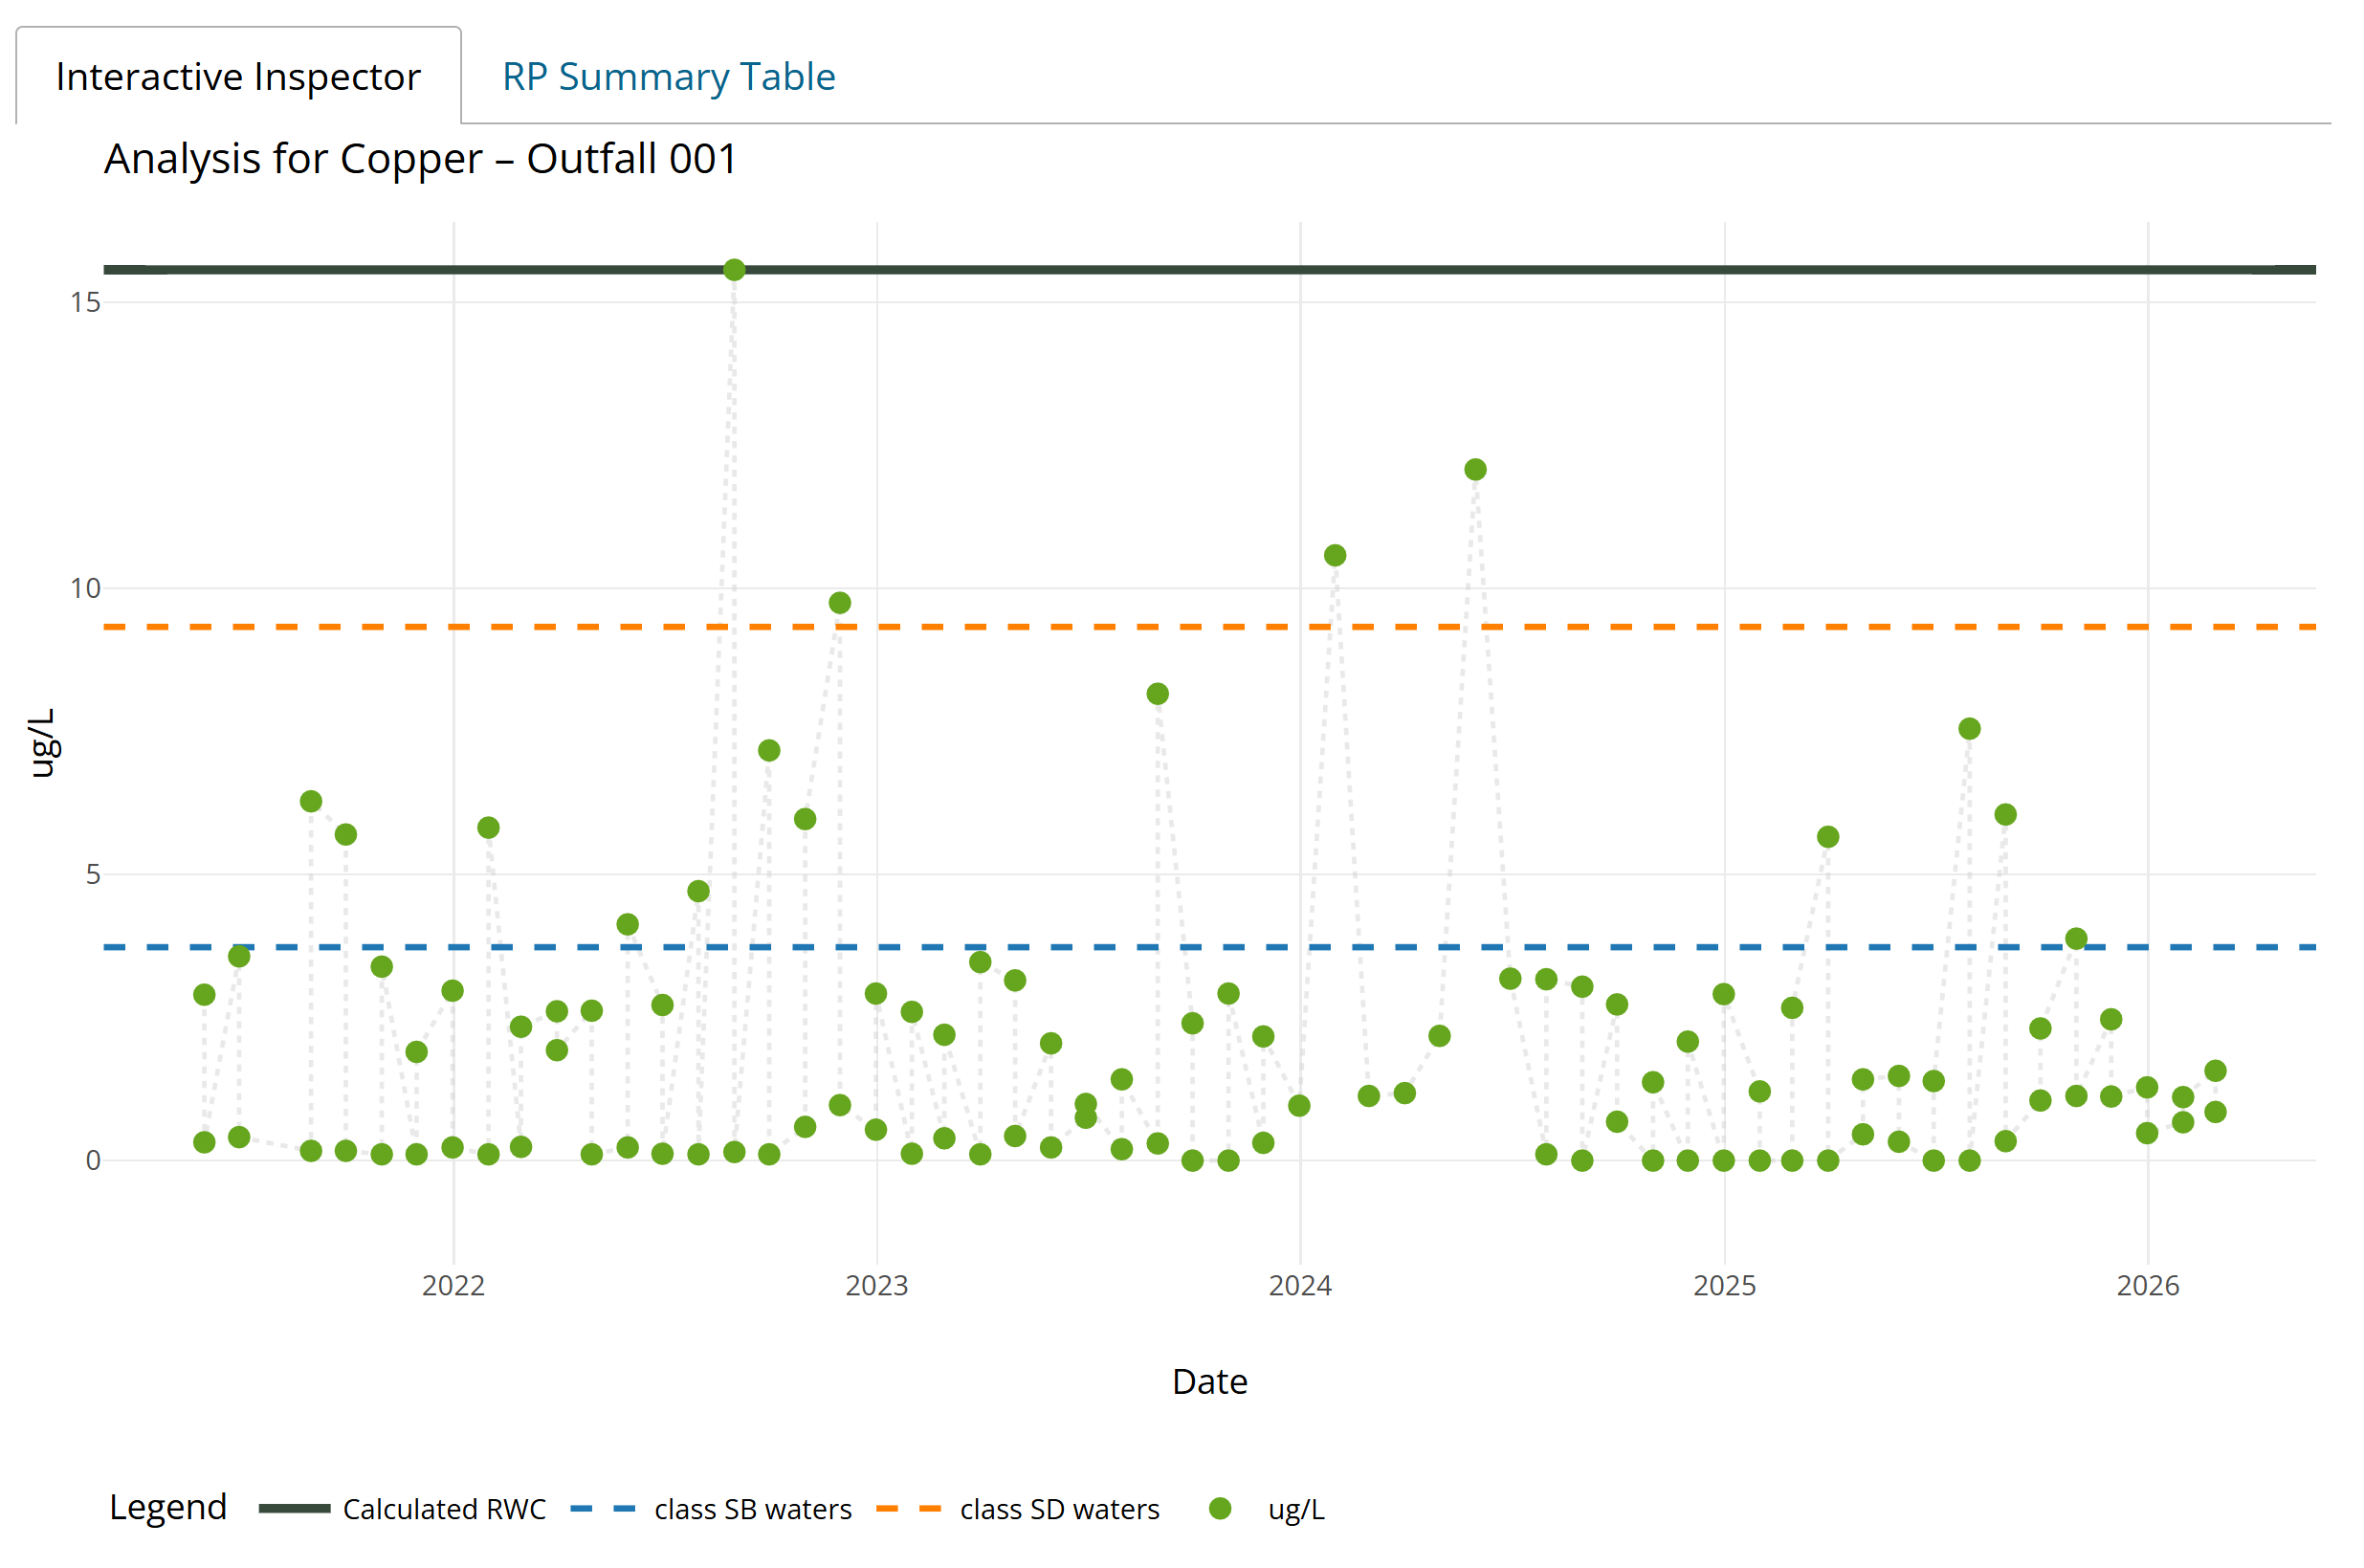
\includegraphics[keepaspectratio]{img/plot_inspector.png}}

}

\caption{Observed vs.~WQS/RWC plot with WQS dashed lines, solid RWC
line, and sample points colored by unit}

\end{figure}%

For hardness-dependent metals in Class SD with the range analysis
active, the plot area gains a second tab, \textbf{Hardness vs Limit},
showing how the criterion varies with hardness and where the critical
hardness falls.

\subsection{The RP Summary Table}\label{sec-summary-table}

The \textbf{RP Summary Table} tab shows the full RP results for the
selected outfall, with one row per pollutant × WQS criterion × water
class combination. Columns include the outfall, WQS criterion ID,
pollutant name, criterion value, unit, water class, the assessed value
(RWC or observed extreme), and the RP determination. Rows are ordered by
RP result --- YES first, then DEPENDS, then NO --- to surface the most
critical findings.

\begin{figure}[H]

{\centering \pandocbounded{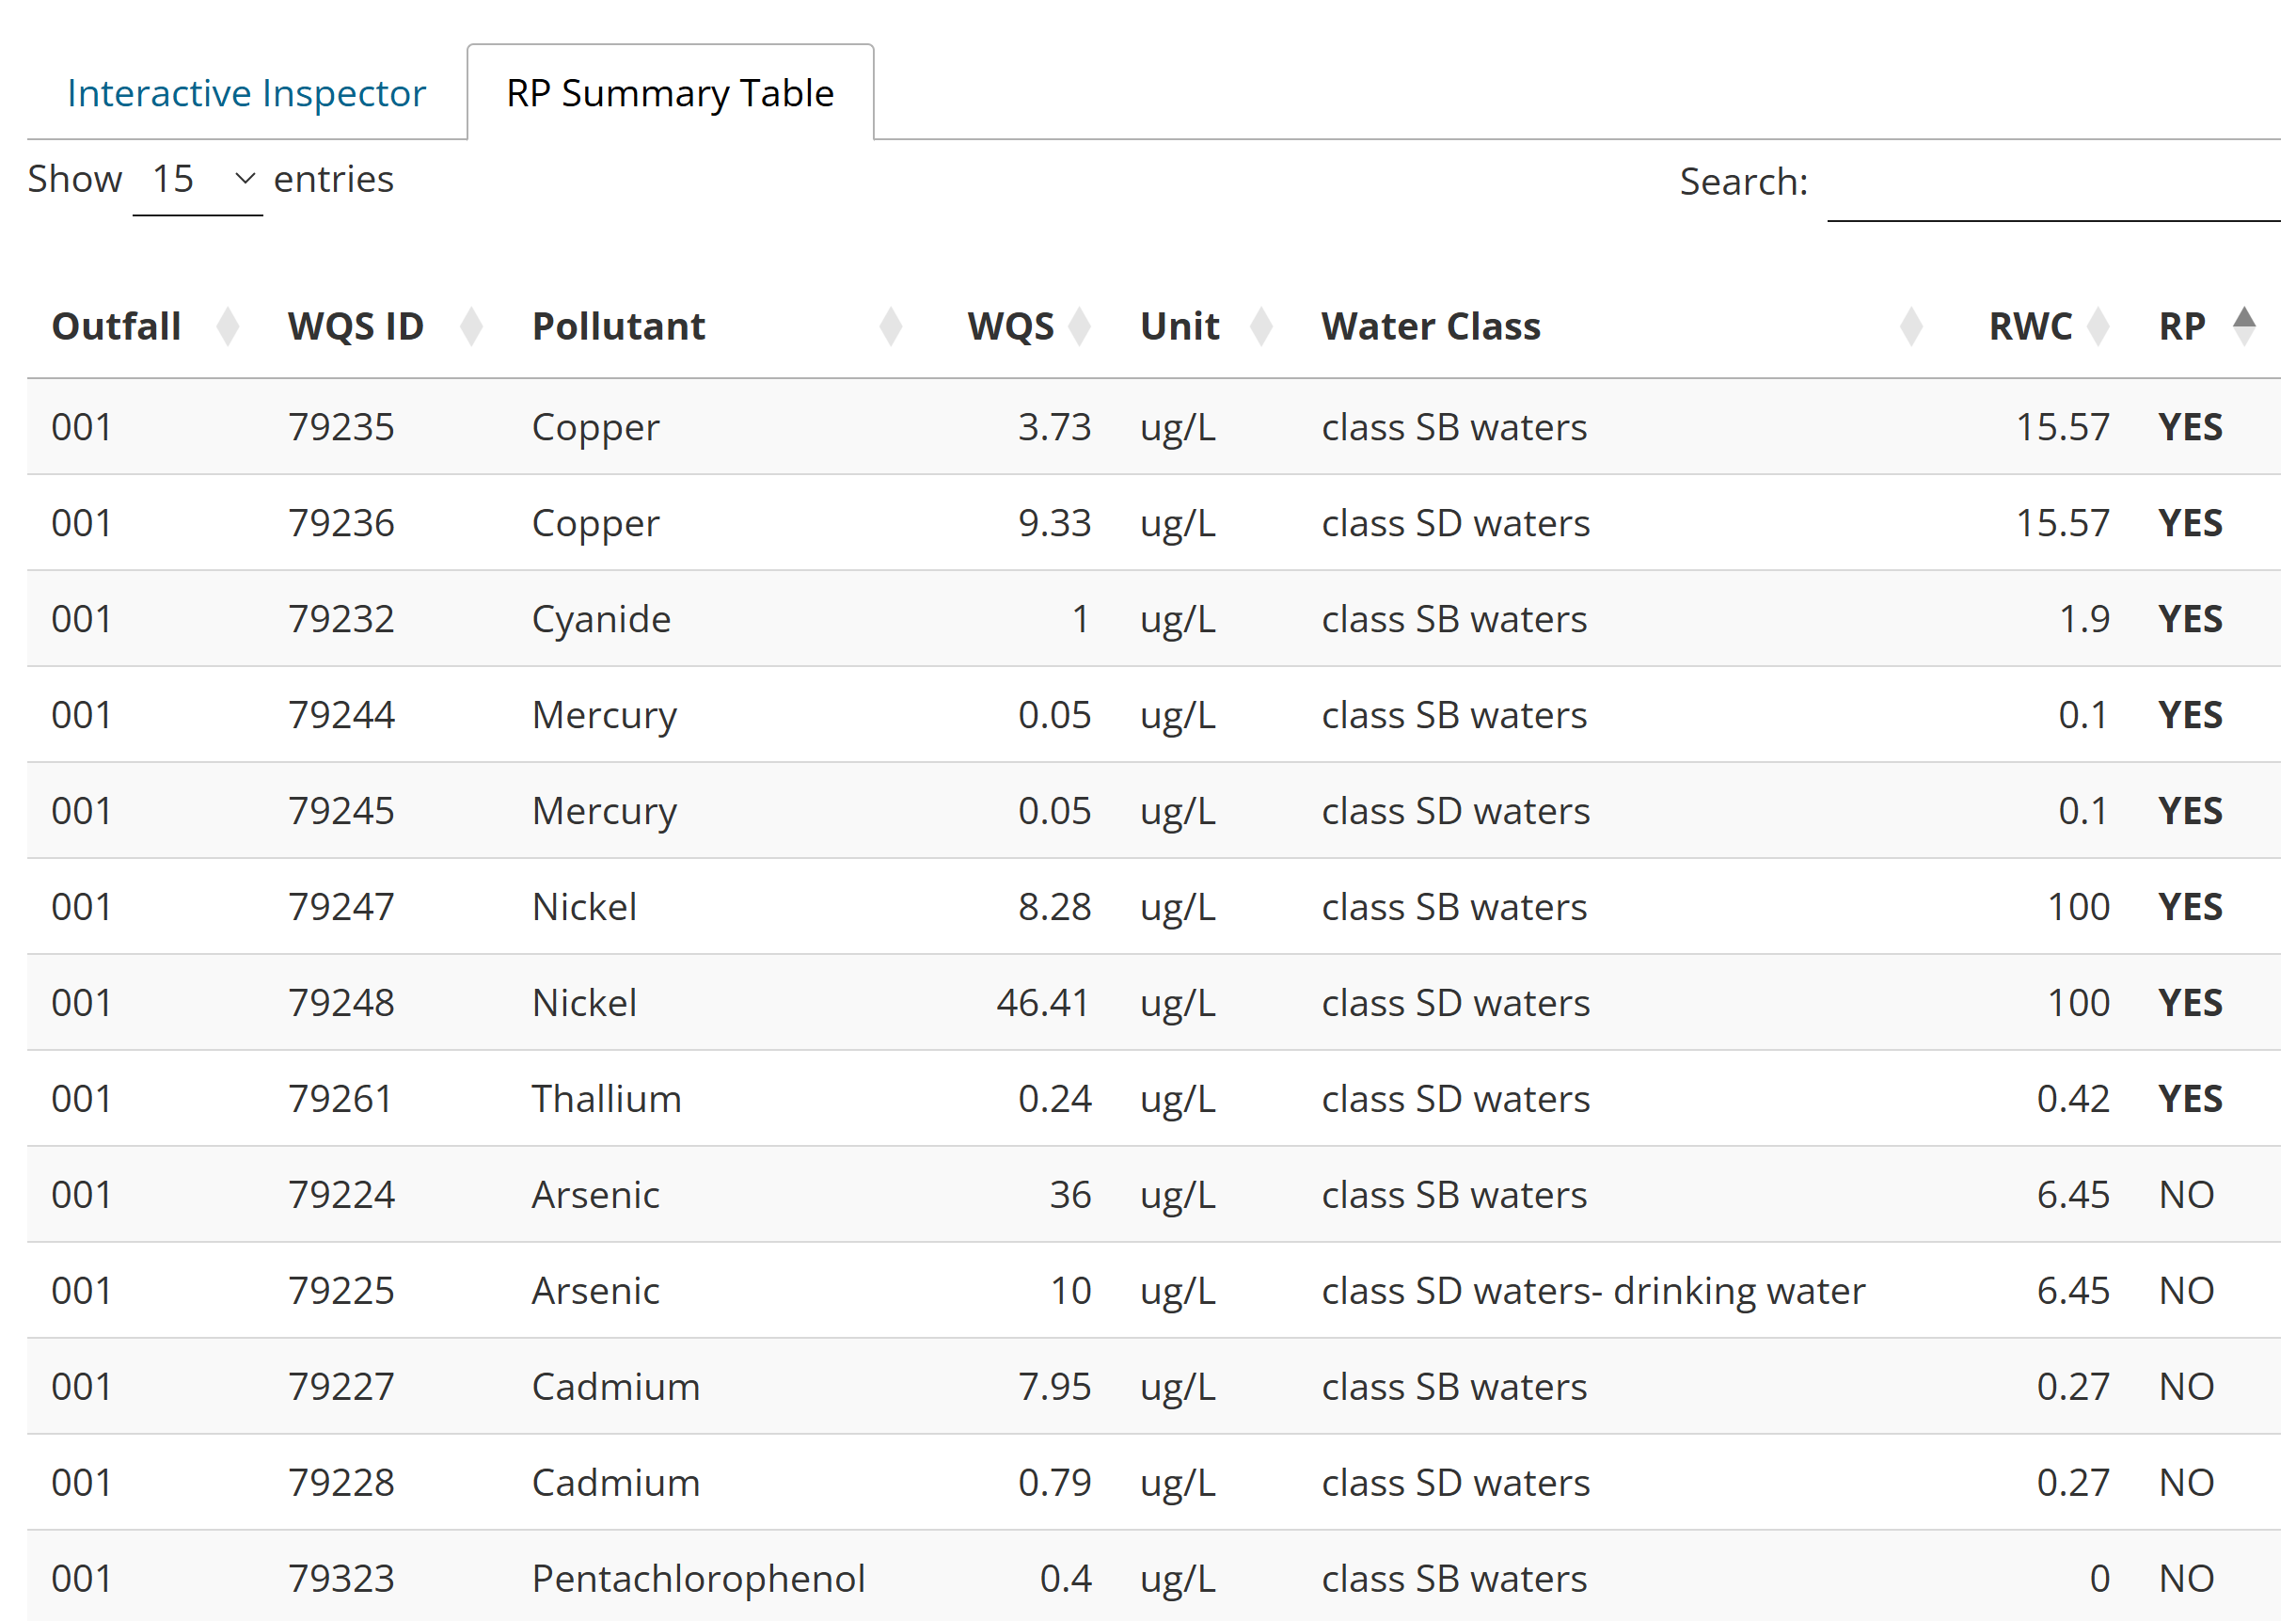
\includegraphics[keepaspectratio]{img/summary_table.png}}

}

\caption{RP Summary Table with YES rows highlighted at top, showing all
columns}

\end{figure}%

\subsection{Direct-Comparison Plots and the Dissolved-Oxygen
Case}\label{sec-do-plot}

Because a floor criterion reads ``backwards'' from a ceiling, the
dissolved-oxygen plot is the clearest illustration of direct comparison:
the criterion is a \textbf{floor} (a value below the line is the
violation), and the observed minimum is what matters. The plot shows the
DO observations against the 5.0 mg/L floor line, with the DO criterion
note visible, and no Calculated RWC line (a DO analysis needs
Streeter-Phelps inputs the app does not carry --- see
Section~\ref{sec-do}).

\begin{figure}[H]

{\centering \pandocbounded{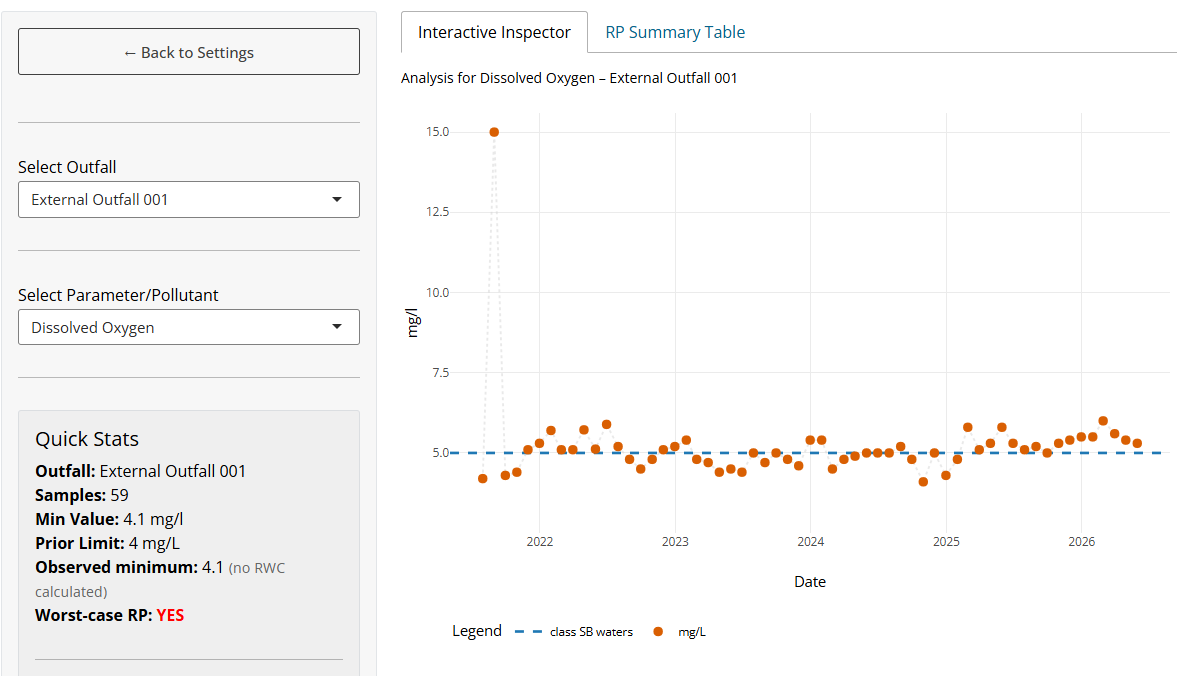
\includegraphics[keepaspectratio]{img/direct_do_plot.png}}

}

\caption{A dissolved-oxygen Inspector plot showing the criterion as a
floor with observations near or below it, and the DO criterion note}

\end{figure}%

\subsection{Log Axis and Non-Detects}\label{sec-log-axis}

When the observed values sit far above a very small criterion, a linear
axis collapses the criterion line onto zero and the plot looks blank.
The app guards against this:

\begin{itemize}
\tightlist
\item
  When the observed maximum is \textbf{100× the criterion or more}, the
  y-axis switches to a log scale and the axis label gains ``(log
  scale).'' This is common and expected rather than a warning about the
  data. Bacteria counts span five or six orders of magnitude by nature,
  and human-health criteria for carcinogens are set far below any
  achievable laboratory quantitation limit --- criteria in the crosswalk
  run down to \(5.1\times10^{-8}\) µg/L for 2,3,7,8-TCDD, so any
  reported detection clears the threshold. A log axis simply keeps the
  criterion line and the observations visible in the same frame.
\item
  Non-detects (NODI codes \textbf{B} and \textbf{Q}) are stored as a
  value of zero, and a log axis cannot display zero. On a log plot they
  are drawn as \textbf{open downward triangles} at a floor equal to the
  smallest positive value in the series, and the plot discloses that
  floor --- in the axis label in the app, and in the figure caption in
  the PDF report. A triangle marks a value known only to be \emph{below}
  the reporting limit; never read it as a measurement.
\item
  If every observation is a non-detect, no positive value exists to
  compare against the criterion, so the plot stays on a linear axis and
  the points render normally at zero.
\end{itemize}

Note that this ratio is \textbf{not} a units check. Reported units are
reconciled against the criterion's units before plotting (see
Section~\ref{sec-interpret-units}), so a wide gap on the plot is not by
itself evidence of a reporting error. The parameters that trigger the
log axis most often --- Enterococci, fecal coliform, sulfide, sulfate
--- are wide-range by nature, and the same log axis and non-detect
markers are mirrored in the PDF report.

\begin{figure}[H]

{\centering \pandocbounded{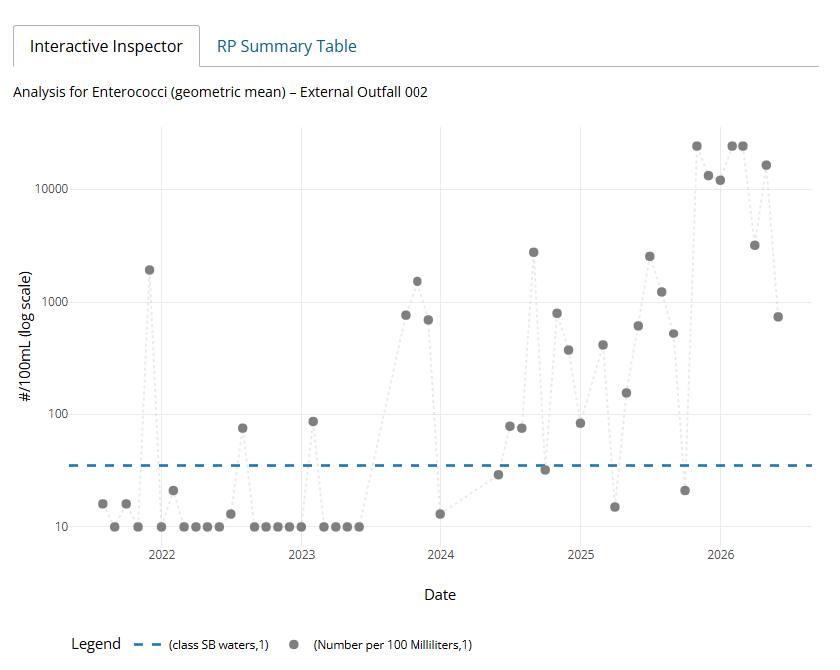
\includegraphics[keepaspectratio]{img/log_axis_flag.png}}

}

\caption{A fecal coliform plot showing the log-scale y-axis and
non-detects drawn as open downward triangles at the plotting floor}

\end{figure}%

\begin{center}\rule{0.5\linewidth}{0.5pt}\end{center}

\section{Report Generation}\label{sec-report}

\subsection{Download Options}\label{sec-download-options}

Click \textbf{Download Report} in the left sidebar of the Findings page.
Two download formats are available:

\textbf{PDF only (default):} A single PDF report rendered from a Quarto
template. The report documents all analysis inputs, settings, and
findings in a format suitable for inclusion in a permit record.

\textbf{PDF + Data (ZIP):} Check the \textbf{Include Data in Download}
checkbox before clicking Download Report. The app bundles the PDF
together with:

\begin{itemize}
\tightlist
\item
  \texttt{data.xlsx} --- an Excel workbook with sheets for the summary
  findings, the full RP results table, the DMR records used in the
  analysis, and the NPDES forms coverage table
\item
  \texttt{README.txt} --- a plain-text summary of the analysis settings
  and permit ID
\end{itemize}

Use the ZIP option when you want to archive the underlying data
alongside the report, or when the findings will be reviewed by others
who need the raw numbers.

\subsection{Report Contents}\label{sec-report-contents}

The PDF report includes:

\textbf{Summary section:} Permit ID, facility name, date range, NPDES
forms, water classifications, dilution ratio, confidence level, target
percentile, hardness setting, and the number of outfalls analyzed. If
the report was produced by Quick Run with unresolved parameters, a
prominent preliminary-report warning appears here.

\textbf{RP Findings table:} All results, ordered by severity (YES, then
DEPENDS, then NO). A \textbf{Basis} column distinguishes ``Calculated''
(a projected RWC) from ``Observed max/min'' (a direct comparison), so an
observed dissolved-oxygen minimum can't be misread as dilution-adjusted.

\textbf{Per-pollutant sections:} One section per pollutant per outfall.
Each section may include:

\begin{itemize}
\tightlist
\item
  An orange \textbf{criterion note} callout at the top of the section,
  carrying the criterion-specific guidance from the crosswalk (the DO
  Streeter-Phelps note, the Enterococci 90-day interval note, the
  temperature in-stream note, or the oil \& grease narrative note)
\item
  A \emph{Reason Included} line and, where applicable, a \emph{Manual
  WQS Applied} callout
\item
  For projected parameters, the step-by-step \textbf{RWC Calculation}
  (\(CV\), \(\sigma_g\), \(p_n\), \(z_p\), \(z_{target}\), MF, RWC)
\item
  For direct-comparison parameters, an \textbf{Assessed Value} note
  stating that the observed maximum or minimum was compared to the
  criterion directly, with no multiplying factor and no dilution ratio
\item
  The observed vs.~WQS/RWC plot (with the same log axis and non-detect
  markers as the app when the values warrant it)
\item
  A limit history table when prior permit limits were present in the DMR
  record
\end{itemize}

\textbf{Manual WQS Overrides and Excluded Parameters:} Sections
documenting any hand-entered criteria and any parameters excluded on the
Needs Attention tab, for the permanent record.

\textbf{Coverage table:} The NPDES forms coverage summary showing which
expected pollutants had data and the unit conversion status for each.

\textbf{Screenshot pending --- \texttt{img/report\_criterion\_note.png}}

An excerpt from a generated PDF report showing an orange criterion-note
callout (the DO Streeter-Phelps note, or the Enterococci interval note)
sitting above the ``Assessed Value'' text in a per-pollutant section.

\begin{figure}[H]

{\centering \pandocbounded{\includegraphics[keepaspectratio]{img/report_criterion_note.png}}

}

\caption{A per-pollutant report section showing the orange
criterion-note callout above the Assessed Value text}

\end{figure}%

\begin{tcolorbox}[enhanced jigsaw, arc=.35mm, bottomrule=.15mm, bottomtitle=1mm, breakable, colback=white, colbacktitle=quarto-callout-note-color!10!white, colframe=quarto-callout-note-color-frame, coltitle=black, left=2mm, leftrule=.75mm, opacityback=0, opacitybacktitle=0.6, rightrule=.15mm, title=\textcolor{quarto-callout-note-color}{\faInfo}\hspace{0.5em}{Note}, titlerule=0mm, toprule=.15mm, toptitle=1mm]

\textbf{Report generation time:} Rendering the PDF runs a Quarto
document with embedded plots for every pollutant × outfall combination.
For facilities with many parameters and multiple outfalls, this can take
30--90 seconds. A progress indicator is displayed during rendering. Do
not close the browser tab while the report is generating.

\end{tcolorbox}

\begin{center}\rule{0.5\linewidth}{0.5pt}\end{center}

\section{Methodology}\label{sec-methodology}

This section describes the statistical and regulatory methods used by
the app to evaluate reasonable potential. It covers the projection
approach used for most parameters, the direct-comparison parameters that
bypass it, the hardness-dependent metals, and Total Ammonia Nitrogen.

\subsection{The Statistical Projection Approach (TSD Section
3.3.2)}\label{sec-statistical-approach}

The fundamental question in an RP determination is whether the effluent,
after accounting for dilution, could cause an exceedance of the
applicable criterion in the receiving water. The challenge is that
effluent concentrations are variable --- a single measured maximum may
not represent the true upper bound of what the discharge is capable of
producing.

EPA's TSD addresses this by treating the effluent concentration data as
a sample from an underlying lognormal distribution and projecting the
upper bound of that distribution at a specified confidence level. This
approach simultaneously accounts for \textbf{data uncertainty} (a small
number of samples represents the highest value less reliably than a
large number does) and estimates the \textbf{statistical upper bound} of
the effluent distribution at a user-specified probability level (the
target percentile). The result is a Multiplying Factor (MF) applied to
the observed maximum concentration before comparing to the criterion.

\subsubsection{The Multiplying Factor}\label{sec-mf}

The MF is derived in two steps following Box 3-2 of the TSD.

\textbf{Step 1 --- Percentile represented by the maximum observation.}
For a dataset of \(n\) samples at confidence level CL, the highest
observed value exceeds the \(p_n\)-th percentile of the underlying
distribution with probability CL, where:

\[p_n = (1 - CL)^{1/n}\]

For example, with \(n = 10\) samples and CL = 0.95, the maximum value
exceeds approximately the 74th percentile of the distribution with 95\%
confidence.

\textbf{Step 2 --- Project from the observed percentile to the target
percentile.} Assuming a lognormal distribution for the effluent:

\[MF = \exp\left[(z_{target} - z_p) \cdot \sigma_g\right]\]

where \(z_{target}\) is the standard normal variate corresponding to the
target percentile, \(z_p\) is the standard normal variate corresponding
to \(p_n\), and \(\sigma_g = \sqrt{\ln(CV^2 + 1)}\) is the geometric
standard deviation of the lognormal distribution expressed via the
coefficient of variation (CV).

The \textbf{coefficient of variation} is estimated as
\(CV = s / \bar{x}\), where \(s\) is the sample standard deviation and
\(\bar{x}\) is the sample mean. For datasets with fewer than 10 samples,
the CV cannot be estimated reliably from the data alone, and the app
assigns a default CV of \textbf{0.6}, consistent with the TSD
recommendation and EPA's national characterization of effluent
variability.

The MF is bounded to be no less than 1. An MF below 1 would imply the
maximum observed value already exceeds the target percentile --- in
which case no upward projection is needed and the maximum value itself
is used.

\subsubsection{The Receiving Water Concentration}\label{sec-rwc}

For projected criteria, the RWC is:

\[RWC = \frac{C_{max} \times MF}{DR}\]

where \(C_{max}\) is the maximum observed effluent concentration (in WQS
units), MF is the multiplying factor, and DR is the dilution ratio. The
RP finding is YES if RWC \textgreater{} criterion for any applicable
water class.

\subsubsection{Worked Example}\label{sec-mf-example}

Consider a facility with 8 observations of a pollutant at an outfall,
with a maximum of 45 µg/L, a mean of 18 µg/L, and a standard deviation
of 12 µg/L. Analysis settings are CL = 0.95, target percentile = 0.95,
and DR = 1. Assume the criterion is 36 µg/L.

\[CV = 12 / 18 = 0.667\]
\[\sigma_g = \sqrt{\ln(0.667^2 + 1)} = \sqrt{\ln(1.444)} = 0.603\]
\[p_n = (1 - 0.95)^{1/8} = 0.05^{0.125} = 0.693\]
\[z_p = \Phi^{-1}(0.693) = 0.503\]
\[z_{target} = \Phi^{-1}(0.95) = 1.645\]
\[MF = \exp\left[(1.645 - 0.503) \times 0.603\right] = \exp(0.689) = 1.99\]
\[RWC = (45 \times 1.99) / 1 = 89.5 \ \mu\text{g/L}\]

Since RWC (89.5 µg/L) \textgreater{} criterion (36 µg/L), the RP
determination is \textbf{YES}. The app displays each intermediate value
--- CV, \(\sigma_g\), \(p_n\), \(z_p\), \(z_{target}\), MF, and RWC ---
in the math inspector on the Interactive Inspector tab.

\subsection{Direct-Comparison Parameters}\label{sec-direct}

Some criteria are not maximum-concentration ceilings and are not
meaningfully projected through the multiplying factor. For these, the
app compares the appropriate observed statistic to the criterion
directly: \textbf{no MF is applied and the dilution ratio is not used.}
Each crosswalk row declares whether it is a ceiling (RP if the value
exceeds the criterion) or a floor (RP if the value falls below it). The
comparison is a \textbf{strict inequality} --- a value exactly on the
criterion is treated as compliant, matching the regulatory wording
(``shall not exceed,'' ``shall not contain less than,'' ``outside the
range of''). A small relative tolerance guards the comparison against
floating-point and unit-conversion noise at the boundary.

Several of these parameters return \textbf{DEPENDS} rather than
\textbf{NO} when no excursion is observed, because a screening-level
end-of-pipe comparison cannot, by itself, rule out reasonable potential.

\subsubsection{pH}\label{sec-ph}

The PRWQSR establishes pH ranges rather than absolute concentration
limits. For Class SD the standard is 6.0--9.0 SU (Rule 1303.2(C)(2)(d));
for Class SB it is 7.3--8.5 SU (Rule 1303.2(B)(2)(d)). pH is evaluated
like any other direct parameter: when the selected water class has a pH
criterion, the app compares the observed pH range to the standard and
reports the result as separate \textbf{\emph{pH (maximum)}} and
\textbf{\emph{pH (minimum)}} rows. An observed maximum at or above the
upper bound, or an observed minimum at or below the lower bound, yields
a \textbf{YES}. This is a direct comparison of observed pH to the
standard, not a statistical RWC projection. pH values are also still
used to compute the TAN criterion (see Section~\ref{sec-tan}). If the
selected class has no pH criterion, pH instead surfaces on the Needs
Attention tab like any other unmatched parameter.

\begin{tcolorbox}[enhanced jigsaw, arc=.35mm, bottomrule=.15mm, bottomtitle=1mm, breakable, colback=white, colbacktitle=quarto-callout-note-color!10!white, colframe=quarto-callout-note-color-frame, coltitle=black, left=2mm, leftrule=.75mm, opacityback=0, opacitybacktitle=0.6, rightrule=.15mm, title=\textcolor{quarto-callout-note-color}{\faInfo}\hspace{0.5em}{Note}, titlerule=0mm, toprule=.15mm, toptitle=1mm]

\textbf{Strict inequality changed some pH results.} Because the
comparison is strict, a pH value sitting exactly on 6.0 or 9.0 is now
treated as compliant. This flips some findings that were previously YES.
This is intended, not a regression --- it reflects the regulatory
language.

\end{tcolorbox}

\subsubsection{Temperature}\label{sec-temperature}

The PRWQSR's thermal standard states that no heat shall be added that
would cause the temperature of \textbf{any site} to exceed 30 °C / 86 °F
(Rule 1303.1(D)(1)). Temperature (00010) is evaluated as a direct
ceiling: \textbf{YES} if the observed maximum exceeds 30 °C,
\textbf{DEPENDS} otherwise. The DEPENDS outcome reflects that this is an
\textbf{in-stream} standard, not an end-of-pipe limit --- an end-of-pipe
comparison is screening only, so the absence of an exceedance at the
pipe does not rule out RP in the receiving water. A note to this effect
is carried into Quick Stats and the report. Temperature appears only
when ``Surface Waters'' or ``All'' is selected (see
Section~\ref{sec-classifications}).

\subsubsection{Dissolved Oxygen}\label{sec-do}

Dissolved oxygen (00300) is a \textbf{floor}: the receiving water must
not fall below 5.0 mg/L, so the compliance-relevant statistic is the
observed \textbf{minimum}, not the maximum. DO is evaluated by direct
comparison --- \textbf{YES} if the observed minimum is below 5.0 mg/L,
\textbf{DEPENDS} otherwise --- and no RWC is calculated.

\begin{tcolorbox}[enhanced jigsaw, arc=.35mm, bottomrule=.15mm, bottomtitle=1mm, breakable, colback=white, colbacktitle=quarto-callout-important-color!10!white, colframe=quarto-callout-important-color-frame, coltitle=black, left=2mm, leftrule=.75mm, opacityback=0, opacitybacktitle=0.6, rightrule=.15mm, title=\textcolor{quarto-callout-important-color}{\faExclamation}\hspace{0.5em}{Important}, titlerule=0mm, toprule=.15mm, toptitle=1mm]

\textbf{Why DO is not projected.} Applying the TSD multiplying factor to
DO is wrong in three ways: it projects an \emph{upper} bound when DO
needs a \emph{lower} bound; the MF is derived for an upper percentile;
and dilution does not attenuate a dissolved-oxygen deficit the way it
attenuates a pollutant. A defensible DO analysis requires the
Streeter-Phelps equation, whose inputs (reaeration and deoxygenation
rates, travel time, upstream deficit) are not present in ICIS-NPDES. The
app therefore screens the observed minimum against the floor and returns
DEPENDS when no excursion is seen, with a note pointing to the
Streeter-Phelps data gap.

\end{tcolorbox}

\subsubsection{Color and Turbidity}\label{sec-color-turbidity}

Color (00080) and turbidity (00070) are direct \textbf{ceilings}: color
at 15 color units (Class SD); turbidity at 50 NTU (Class SD) and 10 NTU
(Class SB). Both are compared directly to the observed maximum. These
parameters previously dropped out of the results entirely because they
were caught in a hardcoded exclusion vector with no downstream handler;
they now flow through the generic direct-comparison path.

\subsubsection{Enterococci}\label{sec-entero}

The PRWQS Enterococci criterion for SB/SD waters is
\textbf{interval-based}: a geometric mean of 35 per 100 mL over any
90-day interval, plus a 90th-percentile criterion of 130 per 100 mL.
These are frequency- and interval-based statistics, not maximum
concentrations, so the multiplying-factor projection is not a meaningful
operation on them. The app splits Enterococci into two direct rows
(geometric mean and 90th percentile) evaluated against their own DMR
statistics, returns \textbf{DEPENDS} when no excursion is observed, and
carries a note instructing the permit writer to evaluate the geometric
mean and 90th percentile over the applicable 90-day intervals
independently. Alternate DMR codes for Enterococci are recognized so the
criterion matches regardless of which code the permittee reported.

\subsubsection{Oil \& Grease}\label{sec-oil}

Oil \& grease is governed by a \textbf{narrative} standard (Rule
1303.1.H): waters shall be substantially free from oils and greases.
There is no numeric value, so the app treats it as a \textbf{binary
detection} test --- any positive reported value triggers RP. Four oil \&
grease method codes are recognized, each carrying its own display label
so they don't collapse into a single confusing entry. As a general
surface-water standard, oil \& grease appears only when ``Surface
Waters'' or ``All'' is selected.

\subsubsection{Surfactants (MBAS)}\label{sec-surfactants}

Surfactants as MBAS carry a numeric standard (SB 500, SD 100 µg/L) and,
for Class SG, a ``shall not be present'' detection standard. The
criterion is recognized under both the methylene-blue-active-substances
code and the surfactants code the permittee may report under, so the
same analyte matches regardless of which code appears in the DMR.

\begin{tcolorbox}[enhanced jigsaw, arc=.35mm, bottomrule=.15mm, bottomtitle=1mm, breakable, colback=white, colbacktitle=quarto-callout-note-color!10!white, colframe=quarto-callout-note-color-frame, coltitle=black, left=2mm, leftrule=.75mm, opacityback=0, opacitybacktitle=0.6, rightrule=.15mm, title=\textcolor{quarto-callout-note-color}{\faInfo}\hspace{0.5em}{Note}, titlerule=0mm, toprule=.15mm, toptitle=1mm]

\textbf{Synonym parameter codes.} A recurring data issue is the same
analyte reported under a DMR code different from the one the criterion
is stored under, which causes a silent non-match. Confirmed cases
(ammonia, Enterococci, surfactants, sulfate) are aligned so the
criterion applies to either code. Other candidates that carry a
regulatory judgment --- e.g., dissolved vs.~total metal fractions,
hexavalent vs.~total chromium --- are deliberately routed to the Needs
Attention tab with a green hint rather than auto-matched, so the permit
writer resolves the distinction.

\end{tcolorbox}

\subsection{Hardness-Dependent Metal Criteria}\label{sec-metals}

Seven metals in Class SD waters have criteria that depend on receiving
water hardness under Rule 1303.1(J)(1) of the PRWQSR. The criterion is a
function of the natural logarithm of hardness expressed in mg/L as
CaCO₃:

\[\text{Criterion} = e^{(LC \cdot \ln(H) - RC)}\]

where \(H\) is the receiving water hardness and \(LC\) and \(RC\) are
regression constants specific to each metal, taken directly from the
PRWQSR footnotes to Table 1 in Rule 1303.1(J)(1):

{\def\LTcaptype{none} % do not increment counter
\begin{longtable}[]{@{}llll@{}}
\toprule\noalign{}
Metal & CRITERION\_ID & LC & RC \\
\midrule\noalign{}
\endhead
\bottomrule\noalign{}
\endlastfoot
Cadmium & 79228 & 0.7977 & 3.909 \\
Chromium III & 79238 & 0.8190 & 0.6848 \\
Copper & 79236 & 0.8545 & 1.702 \\
Lead & 79253 & 1.273 & 4.705 \\
Nickel & 79248 & 0.8460 & 0.0584 \\
Silver & 79251 & 1.72 & 6.59 \\
Zinc & 79264 & 0.8473 & 0.884 \\
\end{longtable}
}

When a specific hardness value is entered, the app computes the
criterion at that hardness and uses it directly in the RP comparison.
When the range analysis option is active, the app computes the
\textbf{critical hardness} --- the hardness at which the criterion would
equal the RWC --- by inverting the formula:

\[H_{critical} = e^{\left(\ln(RWC) + RC\right) / LC}\]

If \(H_{critical}\) is below the plausible range for the receiving water
(e.g., below 25 mg/L as CaCO₃), reasonable potential is unlikely
regardless of hardness. If it is within or above the plausible range,
the permit writer should use a site-specific hardness value to resolve
the determination (see Section~\ref{sec-interpret-depends}).

\subsection{Total Ammonia Nitrogen (TAN)}\label{sec-tan}

Total Ammonia Nitrogen in \textbf{Class SD} surface waters is subject to
a criterion that varies with the pH and temperature of the receiving
water, as specified in Rule 1303.2(C)(2)(l) of the PRWQSR. (TAN is Class
SD only --- there is no Class SB TAN criterion.)

\[TAN = 0.8876 \times \left(\frac{0.0278}{1 + 10^{7.688 - pH}} + \frac{1.1994}{1 + 10^{pH - 7.688}}\right) \times \left(2.126 \times 10^{0.028 \times (20 - T)}\right)\]

where \(T\) is the receiving water temperature in °C and the result is
expressed as mg/L as N. The formula reflects the toxicity of un-ionized
ammonia (NH₃) to aquatic life, which increases as pH and temperature
rise.

\begin{tcolorbox}[enhanced jigsaw, arc=.35mm, bottomrule=.15mm, bottomtitle=1mm, breakable, colback=white, colbacktitle=quarto-callout-warning-color!10!white, colframe=quarto-callout-warning-color-frame, coltitle=black, left=2mm, leftrule=.75mm, opacityback=0, opacitybacktitle=0.6, rightrule=.15mm, title=\textcolor{quarto-callout-warning-color}{\faExclamationTriangle}\hspace{0.5em}{Warning}, titlerule=0mm, toprule=.15mm, toptitle=1mm]

\textbf{Re-run historical TAN determinations.} The leading
\texttt{0.8876} coefficient is required. An earlier inline copy of this
formula in the Run RP handler had dropped it, which inflated every
computed TAN criterion by roughly 12.7\% and made the standard
artificially lenient. The coefficient has been restored. Any TAN
determinations made before this fix should be re-run.

\end{tcolorbox}

\textbf{Parameter codes included.} The app coalesces three
interchangeable ammonia codes into a single total-ammonia-as-N series
before evaluation:

{\def\LTcaptype{none} % do not increment counter
\begin{longtable}[]{@{}lll@{}}
\toprule\noalign{}
Parameter Code & Description & Handling \\
\midrule\noalign{}
\endhead
\bottomrule\noalign{}
\endlastfoot
00610 & Nitrogen, ammonia total {[}as N{]} & Canonical code \\
82230 & Ammonia \& ammonium --- total & Coalesced to 00610 \\
00609 & Ammonia nitrogen, total {[}as N{]} & Coalesced to 00610 \\
\end{longtable}
}

Coalescing 00609 matters in practice: a permit reporting only 00609
previously produced no TAN evaluation at all.

\textbf{Time-varying vs.~fixed limits.} When the app uses pH and
temperature from the DMR (codes 00400 and 00010), the TAN criterion is
computed separately for each monitoring period that has co-occurring pH
and temperature observations, producing a time series of limits. The RP
determination is \textbf{YES} if the TAN RWC exceeds the criterion in
\emph{any} monitoring period (the ``ever crossed'' rule). Summary tables
display the \textbf{mean} TAN limit for readability. When fixed pH and
temperature overrides are used, a single constant TAN limit is computed.
Because the TAN criterion is computed at run time from pH and
temperature rather than stored as a fixed value, TAN is never flagged on
the Needs Attention tab.

\begin{center}\rule{0.5\linewidth}{0.5pt}\end{center}

\section{Interpreting Results and Common
Cases}\label{sec-interpretation}

\subsection{Multiple Water Classes Selected}\label{sec-multi-class}

When more than one water classification is selected, the Observed
vs.~WQS/RWC plot shows a separate dashed criterion line for each class.
The Quick Stats panel shows both the worst-case RP across all classes
and a per-class breakdown. The RP Summary Table lists each class as a
separate row for each pollutant, making it easy to see which classes
drive a YES finding.

A common scenario is selecting both Class SB and Class SD when a
facility may discharge to either coastal or surface receiving waters
depending on the outfall. The more protective of the two criteria drives
the worst-case RP result.

\subsection{Metals with Hardness = Range (Class
SD)}\label{sec-interpret-depends}

When the hardness range analysis is active for a hardness-dependent
metal, the Quick Stats panel shows \textbf{Worst-case RP: DEPENDS}. To
resolve this to a YES or NO, you have two options:

\begin{enumerate}
\def\labelenumi{\arabic{enumi}.}
\tightlist
\item
  \textbf{Use a site-specific hardness value:} Obtain a measured or
  representative hardness value for the receiving water (from ambient
  monitoring, the permit record, or DNER), enter it in the Hardness
  setting, and re-run.
\item
  \textbf{Use the critical hardness threshold:} Read the critical
  hardness annotation from the plot or math inspector. If the critical
  hardness is well above the expected range for the receiving water, a
  NO determination is defensible. Document the basis for the hardness
  assumption in the permit record.
\end{enumerate}

\subsection{Direct-Comparison Parameters Returning
DEPENDS}\label{sec-interpret-direct-depends}

Dissolved oxygen, temperature, and Enterococci return \textbf{DEPENDS}
rather than \textbf{NO} when no excursion is observed. This is
deliberate: for these parameters an end-of-pipe screen cannot rule out
reasonable potential on its own (DO needs a Streeter-Phelps analysis,
temperature is an in-stream standard, and the bacteria criteria are
interval statistics). Treat a DEPENDS here as ``not shown to be a
problem by this screen, but not cleared'' and resolve it with the
additional analysis the criterion note describes.

\subsection{Unit Conversion Issues}\label{sec-interpret-units}

A FAIL or FAIL (Partial) unit status means the app could not convert
some or all reported values to the WQS unit. This does not stop the
analysis --- non-convertible records are dropped from the RP calculation
and values are retained at face value elsewhere --- but the result for
that parameter should be interpreted with caution. Common causes:

\begin{itemize}
\tightlist
\item
  \textbf{Unusual units in the DMR:} Some submissions use non-standard
  unit abbreviations the app does not recognize. If you can confirm the
  unit is equivalent, the face value is correct.
\item
  \textbf{Genuine unit mismatch:} The permittee reported a value in a
  genuinely different unit (e.g., a mass load where a concentration was
  expected). In that case the face value is meaningless and the
  parameter should be flagged for investigation.
\end{itemize}

Note that not every non-PASS status is a data problem. \textbf{EXCLUDED}
means the parameter was reported in a mass-load or flow unit that cannot
be compared to a concentration criterion --- expected for load-based
parameters. \textbf{NO WQS} means there is simply no criterion for the
parameter in the selected class; use the Needs Attention tab to add one
if appropriate. Only \textbf{FAIL} and \textbf{FAIL (Partial)} indicate
an unrecognized unit that warrants investigation.

\subsection{Reading a Log-Scale Plot}\label{sec-interpret-unit-sanity}

A log axis means the observations and the criterion are separated by two
or more orders of magnitude. That is usually real. Bacteria, sulfide,
and sulfate routinely run thousands of times their criteria, and
criteria for PCBs, dioxin, and the chlorinated pesticides sit below what
any laboratory can quantify, so any reported detection clears the
threshold.

Reporting-unit errors do occur, but the app reconciles reported units
against the criterion's units before plotting (see
Section~\ref{sec-interpret-units}), so a wide gap is not by itself
evidence of one. Verify units when a result is surprising for other
reasons --- not because the axis is logarithmic.

Read the open downward triangles with care. They mark non-detects, which
carry no measured value; they are drawn at a plotting floor purely so
they remain visible on a log axis, and the stated floor is the smallest
positive value in that series, not a detection limit reported by the
laboratory. A non-detect is a valid \textbf{NO} finding and the permit
writer needs to see it, but its position on the y-axis carries no
information.

\subsection{No Data for a Parameter}\label{sec-interpret-nodata}

If the selected pollutant has no observations for the selected outfall,
the Inspector shows a ``no data'' message and no row appears in the RP
Summary Table for that combination. This can occur when the parameter
was not monitored at that outfall in the date range, the parameter code
in the crosswalk does not match the code used in the DMR (a synonym-code
issue --- check the Coverage Summary and the Needs Attention hint), or
the data were submitted under a different outfall identifier. A
parameter required by the selected form but with no data appears in the
Coverage Summary with a \textbf{NO DATA} status and a sample count of 0.

\subsection{Prior Limits in the Quick Stats
Panel}\label{sec-prior-limits}

The \textbf{Prior Limit} field shows the most recent numeric effluent
limit from the DMR record for the selected parameter and outfall,
sourced directly from the DMR's limit fields --- it reflects the limit
as recorded in the prior permit, not a limit calculated by this app. It
is provided as a reference point for comparing the current RP analysis
to existing permit conditions.

\begin{center}\rule{0.5\linewidth}{0.5pt}\end{center}

\section{Appendix A: NPDES Application Forms and
Pollutants}\label{sec-appendix-npdes}

The following table lists the pollutants included in the app's crosswalk
by NPDES application form. These are the pollutants for which WQS
criteria exist in the PRWQSR and for which DMR parameter code matches
have been established. Pollutants required by NPDES forms that do not
have a corresponding WQS criterion are tracked in the Coverage Summary;
they are not evaluated for RP automatically, but a criterion can be
supplied for them through the Needs Attention tab (see
Section~\ref{sec-needs-attention}).

\begin{tcolorbox}[enhanced jigsaw, arc=.35mm, bottomrule=.15mm, bottomtitle=1mm, breakable, colback=white, colbacktitle=quarto-callout-note-color!10!white, colframe=quarto-callout-note-color-frame, coltitle=black, left=2mm, leftrule=.75mm, opacityback=0, opacitybacktitle=0.6, rightrule=.15mm, title=\textcolor{quarto-callout-note-color}{\faInfo}\hspace{0.5em}{Note}, titlerule=0mm, toprule=.15mm, toptitle=1mm]

The full crosswalk table is populated from the \texttt{npdes\_forms} and
\texttt{crosswalk} objects loaded at application startup. It carries a
\texttt{sub\_class} column distinguishing stream vs.~reservoir/lake
criteria under Class SD.

\end{tcolorbox}

\begin{center}\rule{0.5\linewidth}{0.5pt}\end{center}

\section{Appendix B: Technical References}\label{sec-appendix-refs}

The following documents provide the regulatory and methodological basis
for the RP Calculator.

\textbf{EPA (1991).} \emph{Technical Support Document for Water
Quality-Based Toxics Control.} EPA/505/2-90-001. Office of Water, U.S.
Environmental Protection Agency, Washington, D.C. Section 3.3.2 ---
Statistical Projection of Upper-Bound Effluent Concentrations.

\textbf{DNER (2025).} \emph{Puerto Rico Water Quality Standards
Regulation, as Amended April 2025.} Resolution R-25-006. Puerto Rico
Department of Natural and Environmental Resources, San Juan, PR. Filed
with the Puerto Rico Department of State June 27, 2025 (Number 9677).

\textbf{40 CFR 122.44(d)(1).} \emph{Conditions applicable to all permits
--- Technology-based and water quality-based effluent limitations.} Code
of Federal Regulations, Title 40, Part 122.

\textbf{40 CFR 131.} \emph{Water Quality Standards.} Code of Federal
Regulations, Title 40, Part 131.

\begin{center}\rule{0.5\linewidth}{0.5pt}\end{center}

\section{Appendix C: Glossary}\label{sec-appendix-glossary}

\textbf{Ceiling criterion:} A criterion the discharge must not exceed.
Reasonable potential exists if the assessed value is above the criterion
(a strict ``greater than'' test).

\textbf{Coefficient of Variation (CV):} The ratio of the standard
deviation to the mean for a dataset, used in the MF calculation as a
measure of relative effluent variability. When \(n < 10\), the app
assigns a default CV of 0.6 per TSD guidance.

\textbf{Confidence Level (CL):} The probability that the highest
observed value in a sample of \(n\) exceeds a given percentile of the
underlying distribution. Defaults to 0.95 (95\%).

\textbf{DEPENDS:} An RP determination returned when no excursion was
observed but the absence of one cannot, by itself, rule out reasonable
potential --- used for hardness-range metals and for direct parameters
such as dissolved oxygen, temperature, and Enterococci.

\textbf{Direct comparison:} Evaluation of a criterion by comparing the
appropriate observed statistic to the criterion value with no
multiplying factor and no dilution ratio. Used for pH, temperature,
dissolved oxygen, color, turbidity, Enterococci, oil \& grease, and
surfactants.

\textbf{DMR (Discharge Monitoring Report):} The periodic report
submitted by NPDES permittees documenting effluent monitoring results.
Sourced by the app from the local ICIS-NPDES database.

\textbf{Dilution Ratio (DR):} The ratio of the total receiving water
flow (including the effluent) to the effluent flow alone at the point of
compliance. Applied only to projected criteria.

\textbf{Floor criterion:} A criterion the receiving water must not fall
below (e.g., dissolved oxygen). Reasonable potential exists if the
assessed value is below the criterion (a strict ``less than'' test); the
compliance-relevant statistic is the observed minimum.

\textbf{ICIS-NPDES:} EPA's Integrated Compliance Information System for
NPDES, the system of record for permit and DMR data. The app reads a
weekly SQLite snapshot of the PR/VI portion of this database, built by
\texttt{refresh\_db.R}.

\textbf{MF (Multiplying Factor):} The statistical factor applied to the
maximum observed effluent concentration to project the upper bound of
the effluent distribution at the target percentile and confidence level.
Bounded to be ≥ 1.

\textbf{NODI Code:} A code in the DMR indicating a reason why no numeric
value was reported for a monitoring period. NODI B and Q (no discharge)
are treated as zero by the app; other NODI codes are excluded.

\textbf{NPDES (National Pollutant Discharge Elimination System):} The
federal permitting program under the Clean Water Act that regulates
point source discharges to waters of the United States.

\textbf{PRWQSR (Puerto Rico Water Quality Standards Regulation):} The
water quality standards regulation administered by DNER. The 2025
amendment is the applicable version in this app.

\textbf{Reasonable Potential (RP):} Under 40 CFR 122.44(d)(1), the
determination that a discharge causes, has the reasonable potential to
cause, or contributes to an excursion above an applicable water quality
standard. A YES RP finding triggers the requirement for a water
quality-based effluent limitation.

\textbf{RWC (Receiving Water Concentration):} For projected criteria,
the projected concentration in the receiving water after accounting for
the statistical upper bound of the effluent distribution and the
available dilution: RWC = (C\_max × MF) ÷ DR. Not calculated for
direct-comparison criteria.

\textbf{Statistic token:} A semantic label (daily maximum, daily
minimum, geometric mean, 90th percentile, average) that governs both
which DMR records are extracted and which value a criterion is compared
against. Raw ICIS statistical-base codes are mapped to these tokens
through a lookup table.

\textbf{TAN (Total Ammonia Nitrogen):} The sum of ammonium ion (NH₄⁺)
and un-ionized ammonia (NH₃). Subject to a pH- and temperature-dependent
criterion in Class SD waters under Rule 1303.2(C)(2)(l).

\textbf{Target Percentile:} The upper bound of the lognormal effluent
distribution that the projected RWC is designed to represent. Defaults
to 0.95 (95th percentile).

\textbf{TSD (Technical Support Document for Water Quality-Based Toxics
Control):} EPA's 1991 guidance document providing the statistical
methodology for RP determinations using effluent monitoring data
(EPA/505/2-90-001).

\textbf{WQS (Water Quality Standards):} A designated use or uses for a
water body, the water quality criteria necessary to protect those uses,
and an antidegradation policy. In this app, WQS refers specifically to
the criteria established in the PRWQSR.




\end{document}
